% =====================================================================
%  Day 2 -- System Dynamics and Control
%  Compile:  TEXINPUTS=../common//: pdflatex -interaction=nonstopmode day2.tex  (twice)
%  Numerical data for some plots: data/*.dat, produced by data/gen_data.py
% =====================================================================
\documentclass[aspectratio=169,10pt]{beamer}
\usetheme{mekatronik}
\setday{2}{System Dynamics and Control}
\title[System Dynamics and Control]{System Dynamics and Control}
\subtitle{Linearisation \textbullet\ Transfer functions \& state space \textbullet\ Identification \textbullet\ PID \textbullet\ Stability}
\author{Mechatronics Training Programme}
\institute{Theoretical Course Series}
\date{Day 2 of 5}

% ------------------------------------------------------------- helpers
\tikzset{
  blk/.style={draw=mkBlue,fill=mkPale,thick,rounded corners=1pt,minimum height=7mm,minimum width=10mm,font=\scriptsize,align=center},
  blko/.style={blk,draw=mkOrange,fill=mkCream},
  sum/.style={draw=mkBlue,thick,circle,inner sep=0pt,minimum size=4mm,fill=white},
  sig/.style={-{Latex[length=2mm]},thick,mkNavy},
  lbl/.style={font=\scriptsize,text=mkNavy},
}
\newcommand{\src}[1]{{\color{mkGray}\fontsize{6}{7}\selectfont [#1]}}

\begin{document}

\begin{frame}[plain]\titlepage\end{frame}

% =====================================================================
\begin{frame}{Agenda and learning objectives}
\begin{columns}[T]
\column{.54\textwidth}
\footnotesize
\begin{tabular}{@{}lp{4.5cm}r@{}}
\toprule
\textbf{Code} & \textbf{Session} & \textbf{Time}\\
\midrule
2.1 & Nonlinear effects and linearisation (cont.) & 0.5\,h\\
2.2 & Transfer functions and state space & 1.0\,h\\
2.3 & System identification and frequency response & 1.0\,h\\
2.4 & PID and basic control structures & 1.5\,h\\
2.5 & Stability and performance analysis & 1.0\,h\\
\midrule
 & \textbf{Net teaching time} (+ short breaks) & \textbf{5.0\,h}\\
\bottomrule
\end{tabular}
\column{.43\textwidth}
\begin{defbox}[After today you can \ldots]
\scriptsize
\checkitem\ linearise a nonlinear servo model about an operating point\\[1pt]
\checkitem\ move freely between $G(s)$, $(A,B,C,D)$ and block diagrams\\[1pt]
\checkitem\ identify FOPDT / 2nd-order models from steps and FRFs\\[1pt]
\checkitem\ tune and implement a practical PID with anti-windup, feedforward and cascades\\[1pt]
\checkitem\ judge stability and robustness via PM, GM, $M_s$, $S$ and $T$
\end{defbox}
\end{columns}
\vspace{2mm}
\begin{notebox}
\textbf{Notation for the whole day:} plant $G(s)$, controller $C(s)$, loop transfer function $L(s)=C(s)G(s)$,
sensitivity $S=1/(1+L)$, complementary sensitivity $T=L/(1+L)$, crossover $\omega_c$, phase margin PM, gain margin GM.
Motor: $R, L_a, k_e, k_t, J, B, T_L$ (armature inductance written $L_a$ to avoid a clash with $L(s)$).
\end{notebox}
\end{frame}

% =====================================================================
\section{2.1 Nonlinear Effects and Linearisation}
% =====================================================================

\begin{frame}{Static nonlinearities in real servo axes}
\begin{columns}[T]
\column{.62\textwidth}
\centering
\begin{tikzpicture}[x=1cm,y=1cm,font=\scriptsize]
  % saturation
  \begin{scope}
    \draw[-{Latex[length=1.5mm]},mkGray] (-1.2,0)--(1.3,0) node[right]{$v$};
    \draw[-{Latex[length=1.5mm]},mkGray] (0,-1.1)--(0,1.2) node[above]{$u$};
    \draw[mkBlue,very thick] (-1.2,-.7)--(-.6,-.7)--(.6,.7)--(1.2,.7);
    \draw[mkOrange,dashed] (.6,0)--(.6,.7) node[pos=0,below]{$v_{\max}$};
    \node[mkNavy,font=\scriptsize\bfseries] at (0,-1.45) {Saturation};
  \end{scope}
  % dead-zone
  \begin{scope}[xshift=3cm]
    \draw[-{Latex[length=1.5mm]},mkGray] (-1.2,0)--(1.3,0) node[right]{$v$};
    \draw[-{Latex[length=1.5mm]},mkGray] (0,-1.1)--(0,1.2) node[above]{$u$};
    \draw[mkBlue,very thick] (-1.2,-.8)--(-.4,0)--(.4,0)--(1.2,.8);
    \draw[mkOrange,<->] (-.4,.15)--(.4,.15) node[midway,above]{$2\delta$};
    \node[mkNavy,font=\scriptsize\bfseries] at (0,-1.45) {Dead-zone};
  \end{scope}
  % backlash
  \begin{scope}[xshift=6cm]
    \draw[-{Latex[length=1.5mm]},mkGray] (-1.2,0)--(1.3,0) node[right]{$\theta_m$};
    \draw[-{Latex[length=1.5mm]},mkGray] (0,-1.1)--(0,1.2) node[above]{$\theta_l$};
    \draw[mkBlue,very thick] (-.6,-.9)--(1.2,.9);
    \draw[mkBlue,very thick] (-1.2,-.9)--(.6,.9);
    \draw[mkBlue,thick,-{Latex[length=1.5mm]}] (.9,.6)--(.3,.6);
    \draw[mkBlue,thick,-{Latex[length=1.5mm]}] (-.9,-.6)--(-.3,-.6);
    \draw[mkOrange,<->] (-1.2,-.95)--(-.6,-.95) node[midway,below]{$2\beta$};
    \node[mkNavy,font=\scriptsize\bfseries] at (0,-1.45) {Backlash (hysteresis)};
\end{scope}
\end{tikzpicture}

\vspace{1mm}
\scriptsize
\begin{tabular}{@{}lll@{}}
\toprule
Nonlinearity & Where in a servo & Typical symptom\\
\midrule
Saturation & DC-link voltage, current limit & windup, slow large steps\\
Dead-zone & IGBT dead-time, valve overlap & distortion near zero, limit cycles\\
Backlash & gears, couplings, belts & position error at reversal, chatter\\
\bottomrule
\end{tabular}
\column{.36\textwidth}
\centering
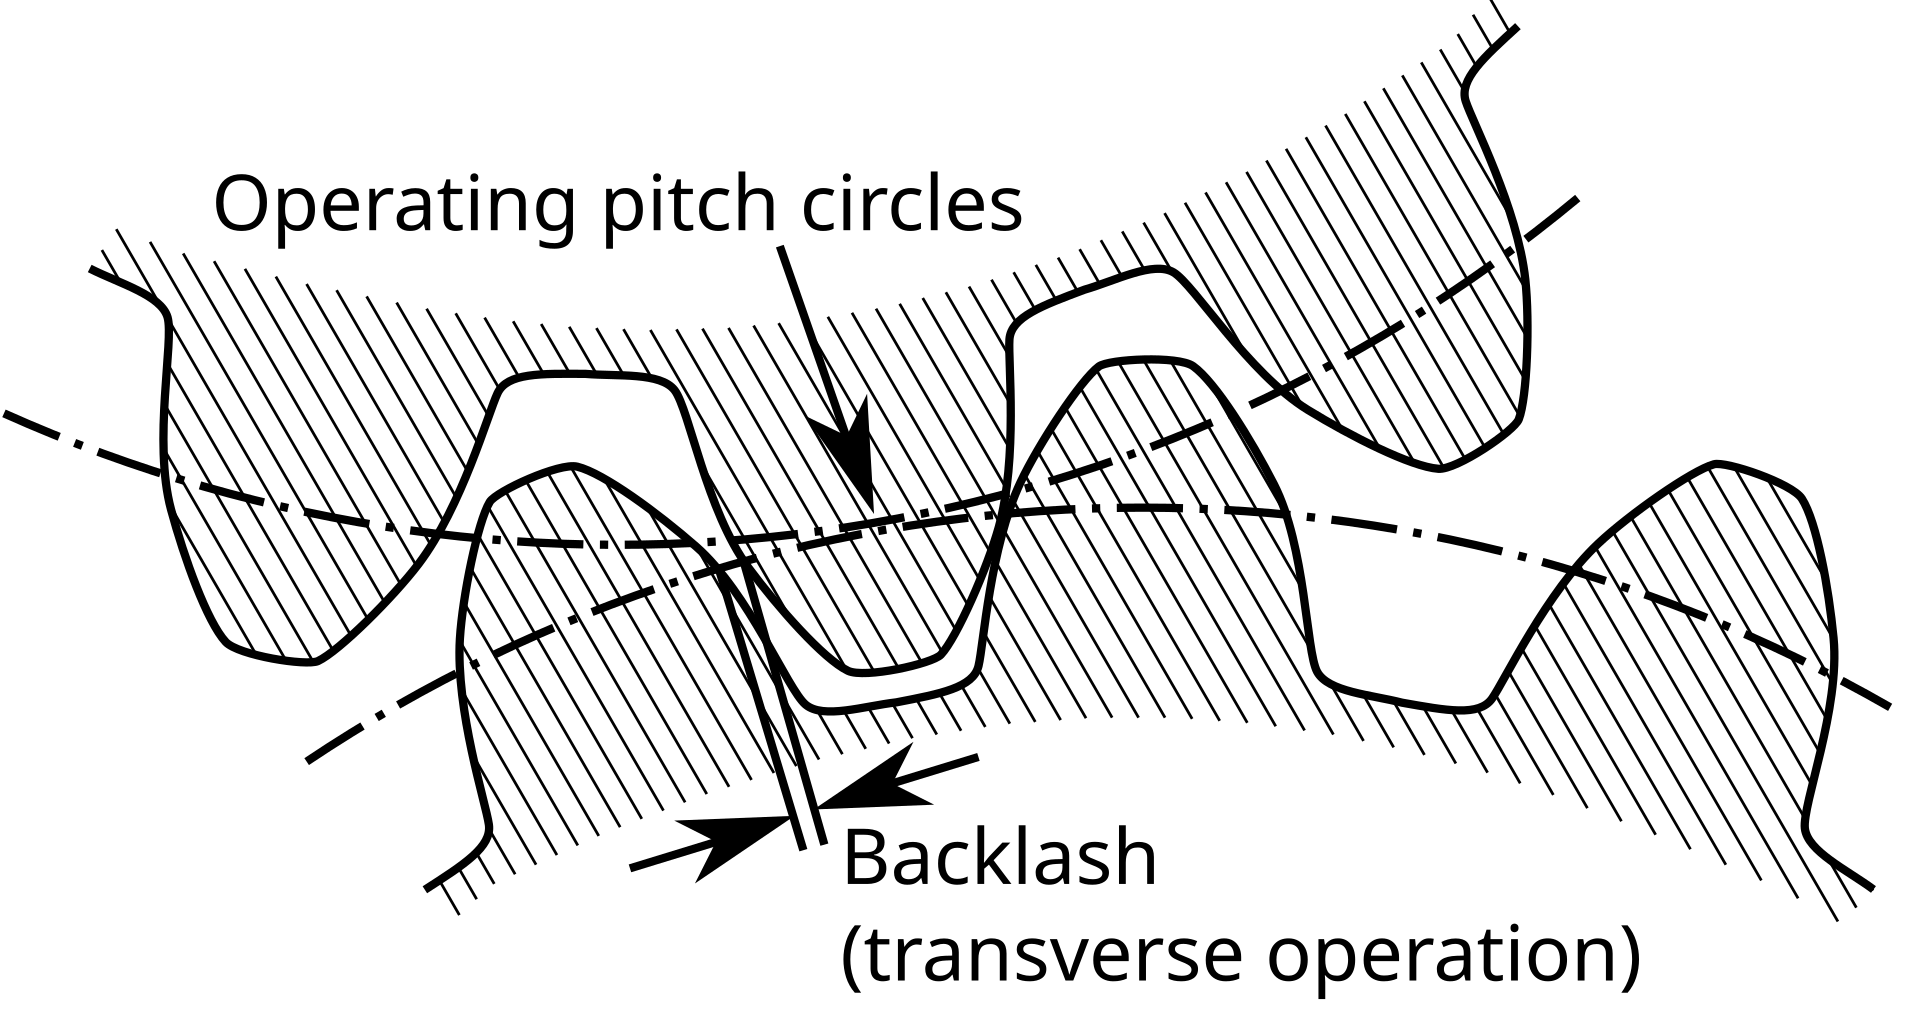
\includegraphics[width=.95\linewidth]{../figures/d2_backlash.png}\\
\credit{GearHeads, Slashme, CC BY-SA 3.0, via Wikimedia Commons}
\vspace{1mm}
\begin{notebox}
\scriptsize\raggedright
Saturation: $u=\operatorname{sat}(v)=\max(-v_{\max},\min(v,v_{\max}))$.\\
Static map $\Rightarrow$ the \term{describing function} $N(A)$ (amplitude-dependent gain) is the classical tool to predict limit cycles [Slotine \& Li, 1991].
\end{notebox}
\end{columns}
\end{frame}

% ---------------------------------------------------------------------
\begin{frame}{Friction: Coulomb, viscous and Stribeck}
\begin{columns}[T]
\column{.5\textwidth}
\centering
\begin{tikzpicture}
\begin{axis}[mkplot,width=6.6cm,height=5.2cm,xlabel={velocity $v$ [mm/s]},ylabel={friction force $F_f$ [N]},
  xmin=-20,xmax=20,ymin=-75,ymax=75,legend pos=north west,axis lines=middle,
  xlabel style={at={(rel axis cs:1,0.5)},anchor=north east},ylabel style={at={(rel axis cs:0.5,1)},anchor=south}]
  \addplot[mkBlue,very thick,domain=0.001:20,samples=150] {(30+(50-30)*exp(-(x/2)^2))+1.2*x};
  \addlegendentry{Stribeck + Coulomb + viscous}
  \addplot[mkBlue,very thick,domain=-20:-0.001,samples=150,forget plot] {-(30+(50-30)*exp(-(x/2)^2))+1.2*x};
  \addplot[mkOrange,thick,dashed,domain=0.001:20] {30+1.2*x}; \addlegendentry{Coulomb + viscous}
  \addplot[mkOrange,thick,dashed,domain=-20:-0.001,forget plot] {-30+1.2*x};
  \addplot[mkSky,thick,dotted,domain=-20:20] {1.2*x}; \addlegendentry{viscous only}
  \draw[mkBlue,very thick] (axis cs:0,-50)--(axis cs:0,50);
  \node[font=\tiny,mkNavy,anchor=west] at (axis cs:0.5,53) {$F_S$};
  \node[font=\tiny,mkNavy,anchor=west] at (axis cs:7,28) {$F_C$};
\end{axis}
\end{tikzpicture}
\column{.48\textwidth}
\begin{eqbox}
\small
\[
F_f(v)=\Big[F_C+(F_S-F_C)\,e^{-(v/v_S)^{2}}\Big]\operatorname{sgn}(v)+B\,v
\]
\end{eqbox}
\scriptsize
\begin{itemize}
  \item $F_S$ static (breakaway), $F_C$ Coulomb level, $v_S$ Stribeck velocity, $B$ viscous coefficient.
  \item At $v=0$ the force is \hl{set-valued} in $[-F_S,F_S]$ (stiction) $\Rightarrow$ non-smooth, not linearisable.
  \item Negative slope $dF_f/dv<0$ at low speed acts as \term{negative damping} $\Rightarrow$ stick--slip.
  \item Integral action + stiction $\Rightarrow$ \hl{hunting limit cycles} around the set-point.
  \item Velocity reversal $\Rightarrow$ \term{quadrant glitches} in contouring (CNC circles).
  \item Remedies: friction feedforward $\hat F_C\operatorname{sgn}(v_{\mathrm{ref}})$, dither, LuGre observer.
\end{itemize}
\src{Armstrong-H\'elouvry, Dupont \& Canudas de Wit, Automatica 1994}
\end{columns}
\end{frame}

% ---------------------------------------------------------------------
\begin{frame}{Magnetic saturation: parameters that depend on the operating point}
\begin{columns}[T]
\column{.5\textwidth}
\centering
\begin{tikzpicture}
\begin{axis}[mkplot,width=6.6cm,height=5.0cm,xlabel={current $i$ [A]},ylabel={$\psi$ [Wb]},
  xmin=0,xmax=30,ymin=0,ymax=0.13,axis y line*=left,ytick={0,0.04,0.08,0.12},
  yticklabel style={/pgf/number format/fixed}]
  \addplot[mkBlue,very thick,domain=0:30,samples=80] {0.12*tanh(x/12)}; \label{pl:psi}
  \addplot[mkBlue,dashed,domain=0:15] {0.01*x};
  \node[font=\tiny,mkBlue,anchor=west] at (axis cs:8.3,0.11) {$L_0 i$ (linear)};
\end{axis}
\begin{axis}[mkplot,width=6.6cm,height=5.0cm,xmin=0,xmax=30,ymin=0,ymax=11,axis y line*=right,axis x line=none,
  ylabel={$L_{\mathrm{inc}}=d\psi/di$ [mH]},grid=none,
  legend style={at={(0.97,0.55)},anchor=east}]
  \addlegendimage{/pgfplots/refstyle=pl:psi}\addlegendentry{flux linkage $\psi(i)$}
  \addplot[mkOrange,very thick,domain=0:30,samples=80] {10/(cosh(x/12))^2};
  \addlegendentry{incremental inductance}
\end{axis}
\end{tikzpicture}
\column{.48\textwidth}
\scriptsize
Iron saturates: $\psi(i)$ bends over and the \term{incremental inductance} falls,
\[
v=R\,i+\frac{d\psi}{dt}=R\,i+L_{\mathrm{inc}}(i)\,\frac{di}{dt},\qquad L_{\mathrm{inc}}=\frac{\partial\psi}{\partial i}.
\]
\begin{itemize}
  \item Current-loop plant $1/(L_{\mathrm{inc}}s+R)$: gain \hl{rises} as $L_{\mathrm{inc}}$ drops
        $\Rightarrow$ crossover moves up, phase margin shrinks at overload.
  \item Torque constant $k_t$ falls at peak current (PMSM: $\psi_{\mathrm{PM}}$ + armature reaction).
  \item Example curve: $\psi=0.12\tanh(i/12)$\,Wb $\Rightarrow L_{\mathrm{inc}}$: 10\,mH at 0\,A, 2.8\,mH at 24\,A.
  \item Practice: gain scheduling $K_p(i)=\hat L_{\mathrm{inc}}(i)\,\omega_{cc}$, or design for the worst case.
\end{itemize}
\end{columns}
\end{frame}

% ---------------------------------------------------------------------
\begin{frame}{Taylor linearisation about an operating point}
\begin{columns}[T]
\column{.52\textwidth}
\scriptsize
Nonlinear model $\dot{\bm x}=\bm f(\bm x,\bm u)$, $\;\bm y=\bm h(\bm x,\bm u)$.\\
Equilibrium (operating point): $\bm f(\bm x_0,\bm u_0)=\bm 0$, $\bm y_0=\bm h(\bm x_0,\bm u_0)$.\\[2pt]
Deviations $\delta\bm x=\bm x-\bm x_0$, $\delta\bm u=\bm u-\bm u_0$; first-order Taylor expansion:
\begin{eqbox}
\[
\delta\dot{\bm x}\approx A\,\delta\bm x+B\,\delta\bm u,\qquad
\delta\bm y\approx C\,\delta\bm x+D\,\delta\bm u
\]
\[
A=\frac{\partial \bm f}{\partial \bm x}\Big|_0,\;
B=\frac{\partial \bm f}{\partial \bm u}\Big|_0,\;
C=\frac{\partial \bm h}{\partial \bm x}\Big|_0,\;
D=\frac{\partial \bm h}{\partial \bm u}\Big|_0
\]
\end{eqbox}
Jacobian entries: $A_{ij}=\partial f_i/\partial x_j$ evaluated at $(\bm x_0,\bm u_0)$.
\column{.45\textwidth}
\begin{keybox}[Validity -- Lyapunov's indirect method]
\scriptsize
\begin{itemize}
  \item All eigenvalues of $A$ in the open LHP $\Rightarrow$ equilibrium \hl{locally} asymptotically stable.
  \item Any eigenvalue in the RHP $\Rightarrow$ unstable.
  \item Eigenvalue on the $j\omega$-axis $\Rightarrow$ no conclusion from the linear model.
\end{itemize}
\end{keybox}
\begin{notebox}
\scriptsize
Not applicable at non-smooth points (Coulomb friction at $v=0$, backlash, saturation corner): use describing functions or simulation.
A family of linear models over operating points $\Rightarrow$ \term{gain scheduling}.
\end{notebox}
\end{columns}
\end{frame}

% ---------------------------------------------------------------------
\begin{frame}{Example 1: pendulum / unbalanced arm on a servo motor}
\begin{columns}[T]
\column{.25\textwidth}
\centering
\begin{tikzpicture}[scale=.9]
  \fill[pattern=north east lines,pattern color=mkGray] (-1,0) rectangle (1,.2);
  \draw[thick,mkGray] (-1,0)--(1,0);
  \draw[dashed,mkGray] (0,0)--(0,-2.6);
  \draw[very thick,mkBlue] (0,0)--({2.2*sin(30)},{-2.2*cos(30)}) coordinate (m);
  \fill[mkOrange] (m) circle (.17);
  \fill[mkNavy] (0,0) circle (.06);
  \draw[->,mkOrange,thick] (0,-1.1) arc (-90:-60:1.1) node[pos=.6,below]{\scriptsize$\theta$};
  \draw[-{Latex},thick,mkMid] (m)--++(0,-.8) node[right]{\scriptsize$mg$};
  \draw[-{Latex},thick,mkNavy] (-.35,.45) arc (150:30:.4) node[right]{\scriptsize$\tau$};
  \node[font=\scriptsize] at (.4,-1.5) {$l$};
\end{tikzpicture}
\column{.37\textwidth}
\scriptsize
$J\ddot\theta=\tau-mgl\sin\theta-b\dot\theta$, $\;\bm x=[\theta,\ \dot\theta]^{\!\top}$, $u=\tau$.
\[
A=\begin{bmatrix}0&1\\-\tfrac{mgl}{J}\cos\theta_0&-\tfrac{b}{J}\end{bmatrix},\;
B=\begin{bmatrix}0\\ \tfrac1J\end{bmatrix}
\]
\textbf{Hanging} $\theta_0=0$: $\lambda^2+\tfrac bJ\lambda+\tfrac{mgl}J=0$ $\Rightarrow$ stable, $\omega_n=\sqrt{mgl/J}$.\\[2pt]
\textbf{Inverted} $\theta_0=\pi$: $\lambda^2+\tfrac bJ\lambda-\tfrac{mgl}J=0$ $\Rightarrow$ one \hl{RHP pole}.\\[2pt]
Numbers: $m=2$\,kg, $l=0.3$\,m, $J=ml^2=0.18$\,kg\,m$^2$ $\Rightarrow\omega_n=\sqrt{g/l}=5.72$\,rad/s (0.91\,Hz).
Torque needed to hold $\theta_0$: $\tau_0=mgl\sin\theta_0$ (max 5.9\,Nm).
\column{.36\textwidth}
\centering
\begin{tikzpicture}
\begin{axis}[mkplot,width=5.4cm,height=4.6cm,xlabel={$\theta$ [deg]},ylabel={$\sin\theta$},
  xmin=-30,xmax=210,ymin=-1.3,ymax=1.3,xtick={0,90,180},legend pos=south west,legend columns=1]
  \addplot[mkBlue,very thick,domain=-30:210,samples=100] {sin(x)}; \addlegendentry{$\sin\theta$}
  \addplot[mkOrange,thick,dashed,domain=-30:75] {rad(x)}; \addlegendentry{lin.\ at $0$}
  \addplot[mkMid,thick,dashed,domain=105:210] {-rad(x-180)}; \addlegendentry{lin.\ at $\pi$}
  \fill[mkOrange] (axis cs:0,0) circle (1.6pt);\fill[mkMid] (axis cs:180,0) circle (1.6pt);
\end{axis}
\end{tikzpicture}\\
\scriptsize Error of $\sin\theta\approx\theta$: 1\,\% at 14$^\circ$, 5\,\% at 31$^\circ$.
\end{columns}
\end{frame}

% ---------------------------------------------------------------------
\begin{frame}{Example 2: electromagnet (magnetic levitation / actuator)}
\begin{columns}[T]
\column{.28\textwidth}
\centering
\begin{tikzpicture}[scale=.85]
  \fill[mkGray!60] (-1,1.4) rectangle (1,2);
  \fill[mkGray!60] (-1,0.5) rectangle (-.6,1.4);\fill[mkGray!60] (.6,0.5) rectangle (1,1.4);
  \fill[mkGray!60] (-.2,0.5) rectangle (.2,1.4);
  \foreach \y in {0.65,0.85,1.05,1.25}{\draw[mkOrange,thick] (-.55,\y)--(-.25,\y); \draw[mkOrange,thick] (.25,\y)--(.55,\y);}
  \fill[mkBlue] (-.9,-.6) rectangle (.9,-.25);
  \draw[<->,mkNavy] (1.2,0.5)--(1.2,-.25) node[midway,right]{\scriptsize$z$};
  \draw[-{Latex},thick,mkMid] (0,-.6)--(0,-1.3) node[right]{\scriptsize$mg$};
  \draw[-{Latex},thick,mkOrange] (-.5,-.25)--(-.5,.3) node[left]{\scriptsize$F$};
  \node[font=\scriptsize] at (-1.4,1) {$i$};
\end{tikzpicture}\\[1mm]
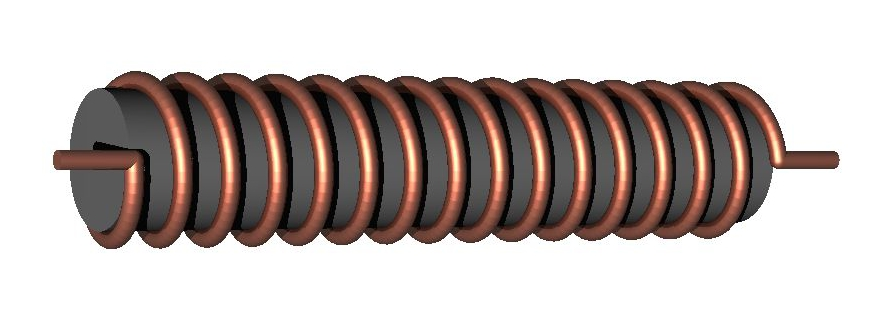
\includegraphics[width=.95\linewidth]{../figures/d2_solenoid.jpg}\\
\credit{Svjo, CC BY-SA 3.0, via Wikimedia Commons}
\column{.70\textwidth}
\scriptsize
Force (ideal magnetic circuit, gap $z$ measured downward): $F=k\,i^2/z^2$, \quad $m\ddot z=mg-k\,i^2/z^2$.\\
Equilibrium: $i_0=z_0\sqrt{mg/k}$. Linearise $F(i,z)$:
\begin{eqbox}
\[
\delta F=\underbrace{\frac{2k i_0}{z_0^2}}_{K_i}\delta i-\underbrace{\frac{2k i_0^2}{z_0^3}}_{K_z}\delta z
\;\Rightarrow\;
m\,\delta\ddot z=K_z\,\delta z-K_i\,\delta i,\qquad
\frac{\delta Z(s)}{\delta I(s)}=\frac{-K_i}{m s^2-K_z}
\]
\end{eqbox}
\textbf{Worked example:} $m=0.1$\,kg, $z_0=5$\,mm, $i_0=1$\,A $\Rightarrow k=mgz_0^2/i_0^2=2.45\times10^{-5}$\,N\,m$^2$/A$^2$.
\begin{itemize}
  \item $K_z=2mg/z_0=392$\,N/m (\hl{negative stiffness}), $K_i=2mg/i_0=1.96$\,N/A.
  \item Poles $s=\pm\sqrt{K_z/m}=\pm62.6$\,rad/s $\Rightarrow$ open-loop unstable, time constant 16\,ms.
  \item Both gains scale with the operating point: $K_z\propto 1/z_0$, $K_i\propto 1/i_0$ $\Rightarrow$ the linear model is valid only near $(z_0,i_0)$.
\end{itemize}
Same structure appears in magnetic bearings and in reluctance actuators.
\end{columns}
\end{frame}

% ---------------------------------------------------------------------
\begin{frame}{Session 2.1 -- Summary}
\begin{keybox}[Key take-aways]
\begin{itemize}
  \item Servo axes contain saturation, dead-zone, backlash, friction and magnetic saturation; they set the
        limits of what linear control can do.
  \item Friction has a \hl{set-valued} stiction part and a negative-damping Stribeck part: cause of stick--slip and hunting.
  \item Smooth nonlinearities are handled by \term{Jacobian linearisation} around an equilibrium $(\bm x_0,\bm u_0)$.
  \item The linear model is \hl{local}: gains and even stability (pendulum up/down, maglev) depend on the operating point.
  \item Non-smooth effects need describing functions, compensation (feedforward) or simulation.
\end{itemize}
\end{keybox}
\begin{notebox}
Next: having a linear model, we describe it compactly by a transfer function or a state-space model.
\end{notebox}
\end{frame}

% =====================================================================
\section{2.2 Transfer Functions and State Space}
% =====================================================================

\begin{frame}{Laplace transform, transfer function, poles and zeros}
\begin{columns}[T]
\column{.5\textwidth}
\scriptsize
$F(s)=\int_0^\infty f(t)e^{-st}dt$ turns linear ODEs into algebra:\\[2pt]
\begin{tabular}{@{}ll@{}}
\toprule
Time domain & Laplace domain\\
\midrule
$\dot f(t)$ & $sF(s)-f(0)$\\
$\int_0^t f\,d\tau$ & $F(s)/s$\\
$f(t-T_d)$ (delay) & $e^{-sT_d}F(s)$\\
convolution $g*u$ & $G(s)U(s)$\\
$f(\infty)$ (if it exists) & $\lim_{s\to0}sF(s)$\\
\bottomrule
\end{tabular}\\[3pt]
With zero initial conditions:
\begin{eqbox}
\[
G(s)=\frac{Y(s)}{U(s)}=\frac{b_ms^m+\dots+b_0}{s^n+a_{n-1}s^{n-1}+\dots+a_0}
=K\frac{\prod_i(s-z_i)}{\prod_j(s-p_j)}
\]
\end{eqbox}
\begin{itemize}
  \item \term{Order} $n$ = number of poles = number of energy stores.
  \item \term{Relative degree} $n-m$: proper if $m\le n$ (physical plants: $m<n$).
\end{itemize}
\column{.47\textwidth}
\centering
\begin{tikzpicture}[scale=.85]
  \fill[mkCream] (0,-2.2) rectangle (2.2,2.2);
  \node[font=\tiny,mkOrange,anchor=north east] at (2.2,2.2) {unstable (RHP)};
  \fill[mkPale] (-4,-2.2) rectangle (0,2.2);
  \node[font=\tiny,mkBlue,anchor=north west] at (-4,2.2) {stable (LHP)};
  \draw[-{Latex},mkGray] (-4,0)--(2.4,0) node[right]{\scriptsize Re};
  \draw[-{Latex},mkGray] (0,-2.3)--(0,2.4) node[above]{\scriptsize Im};
  \foreach \p in {(-1,1.5),(-1,-1.5),(-3,0)}{\draw[mkBlue,very thick] \p++(-.12,-.12)--++(.24,.24) \p++(-.12,.12)--++(.24,-.24);}
  \draw[mkOrange,very thick] (-2,0) circle (.12);
  \draw[mkOrange,very thick] (1,0) circle (.12);
  \node[font=\tiny,above] at (-1,1.6) {pole};
  \node[font=\tiny,below] at (-2,-0.12) {zero};
  \node[font=\tiny,below,align=center] at (1,-.12) {RHP zero\\(non-min.\ phase)};
\end{tikzpicture}\\
\scriptsize
\begin{itemize}
  \item \hl{Poles} (roots of denominator) set the \emph{modes} $e^{p_jt}$: stability and speed.
  \item \hl{Zeros} set how the modes are \emph{weighted}; RHP zeros cause undershoot and limit bandwidth.
  \item DC gain $G(0)$; time delay $e^{-sT_d}$ is not rational (Pad\'e approximation).
\end{itemize}
\end{columns}
\end{frame}

% ---------------------------------------------------------------------
\begin{frame}{First-order system}
\begin{columns}[T]
\column{.55\textwidth}
\centering
\begin{tikzpicture}
\begin{axis}[mkplot,width=7.6cm,height=5.0cm,xlabel={$t/\tau$},ylabel={$y(t)/(K u_0)$},
  xmin=0,xmax=5,ymin=0,ymax=1.1,xtick={0,1,2,3,4,5},ytick={0,0.632,0.865,0.95,0.98,1},
  yticklabel style={/pgf/number format/fixed}]
  \addplot[mkBlue,very thick,domain=0:5,samples=100] {1-exp(-x)};
  \addplot[mkOrange,thick,dashed,domain=0:1.05] {x};
  \draw[mkGray,dashed] (axis cs:1,0)--(axis cs:1,0.632)--(axis cs:0,0.632);
  \draw[mkGray,dashed] (axis cs:3,0)--(axis cs:3,0.95);
  \node[font=\tiny,anchor=west,mkOrange] at (axis cs:1.05,0.98) {initial slope $1/\tau$};
  \node[font=\tiny,anchor=west] at (axis cs:1.05,0.58) {63.2\,\% at $t=\tau$};
  \node[font=\tiny,anchor=west] at (axis cs:3.05,0.9) {95\,\% at $3\tau$};
\end{axis}
\end{tikzpicture}
\column{.43\textwidth}
\begin{eqbox}
\[
G(s)=\frac{K}{\tau s+1},\quad y(t)=Ku_0\big(1-e^{-t/\tau}\big)
\]
\end{eqbox}
\scriptsize
\begin{itemize}
  \item One pole at $s=-1/\tau$; bandwidth $\omega_b=1/\tau$ (\SI{-3}{dB}).
  \item 10--90\,\% rise time $t_r=2.2\tau$; 2\,\% settling $t_s\approx4\tau$.
  \item No overshoot, no oscillation -- ever.
\end{itemize}
\textbf{Servo examples}
\begin{itemize}
  \item R--L winding: $I/V=1/(L_as+R)$, $\tau_e=L_a/R$.
  \item Inertia with viscous friction: $\Omega/T=1/(Js+B)$, $\tau=J/B$.
  \item A well-tuned closed current loop $\approx 1/(\tau_{cl}s+1)$ seen from the speed loop.
\end{itemize}
\end{columns}
\end{frame}

% ---------------------------------------------------------------------
\begin{frame}{Second-order standard form and pole geometry}
\begin{columns}[T]
\column{.5\textwidth}
\begin{eqbox}
\[
G(s)=\frac{K\,\omega_n^2}{s^2+2\zeta\omega_n s+\omega_n^2}
\]
\end{eqbox}
\scriptsize
\begin{itemize}
  \item $\omega_n$ natural frequency [rad/s], $\zeta$ damping ratio [--].
  \item Poles $p_{1,2}=-\zeta\omega_n\pm j\omega_n\sqrt{1-\zeta^2}=-\sigma\pm j\omega_d$.
  \item $|p|=\omega_n$ (distance from origin), $\cos\varphi=\zeta$ (angle to the negative real axis).
  \item $\zeta<1$ underdamped, $\zeta=1$ critically damped, $\zeta>1$ overdamped (two real poles).
  \item Mechanical analogue: $m\ddot x+c\dot x+kx=F$ $\Rightarrow$ $\omega_n=\sqrt{k/m}$, $\zeta=c/(2\sqrt{km})$.
\end{itemize}
\column{.47\textwidth}
\centering
\begin{tikzpicture}[scale=1.0]
  \draw[-{Latex},mkGray] (-3.3,0)--(1,0) node[right]{\scriptsize Re};
  \draw[-{Latex},mkGray] (0,-2.4)--(0,2.5) node[above]{\scriptsize Im};
  \draw[mkSky,dashed] (0,0) circle (2.3);
  \coordinate (p) at ({-2.3*cos(50)},{2.3*sin(50)});
  \coordinate (q) at ({-2.3*cos(50)},{-2.3*sin(50)});
  \draw[mkBlue,thick] (0,0)--(p) node[midway,above right,font=\scriptsize]{$\omega_n$};
  \draw[mkBlue,thick] (0,0)--(q);
  \foreach \c in {p,q}{\draw[mkOrange,very thick] (\c)++(-.13,-.13)--++(.26,.26) (\c)++(-.13,.13)--++(.26,-.26);}
  \draw[mkGray,dashed] (p)--(0,{2.3*sin(50)}) node[right,font=\scriptsize]{$\omega_d$};
  \draw[mkGray,dashed] (p)--({-2.3*cos(50)},0) node[below,font=\scriptsize]{$-\sigma=-\zeta\omega_n$};
  \draw[mkOrange,thick] (-.8,0) arc (180:130:.8);
  \node[font=\scriptsize,mkOrange] at (-.95,.45) {$\varphi$};
  \node[font=\tiny,align=center,mkNavy] at (-2.3,-1.9) {constant-$\zeta$ ray\\$\zeta=\cos\varphi$};
\end{tikzpicture}
\end{columns}
\end{frame}

% ---------------------------------------------------------------------
\begin{frame}{Step responses of the second-order system for different $\zeta$}
\begin{columns}[T]
\column{.62\textwidth}
\centering
\begin{tikzpicture}
\begin{axis}[mkplot,width=8.6cm,height=5.8cm,xlabel={normalised time $\omega_n t$},ylabel={$y(t)/K$},
  xmin=0,xmax=16,ymin=0,ymax=1.85,legend pos=north east,legend columns=2,
  cycle list={{mkRed,thick},{mkOrange,thick},{mkAmber,thick},{mkBlue,very thick},{mkMid,thick,dashed},{mkSky,thick,dotted}}]
  \addplot+[domain=0:16,samples=220] {1-exp(-0.1*x)/sqrt(1-0.01)*sin(deg(sqrt(1-0.01)*x)+acos(0.1))}; \addlegendentry{$\zeta=0.1$}
  \addplot+[domain=0:16,samples=200] {1-exp(-0.3*x)/sqrt(1-0.09)*sin(deg(sqrt(1-0.09)*x)+acos(0.3))}; \addlegendentry{$\zeta=0.3$}
  \addplot+[domain=0:16,samples=200] {1-exp(-0.5*x)/sqrt(1-0.25)*sin(deg(sqrt(1-0.25)*x)+acos(0.5))}; \addlegendentry{$\zeta=0.5$}
  \addplot+[domain=0:16,samples=200] {1-exp(-0.707*x)/sqrt(1-0.5)*sin(deg(sqrt(1-0.5)*x)+acos(0.707))}; \addlegendentry{$\zeta=0.707$}
  \addplot+[domain=0:16,samples=200] {1-(1+x)*exp(-x)}; \addlegendentry{$\zeta=1$}
  \addplot+[domain=0:16,samples=200] {1+(-3.7321*exp(-0.26795*x)+0.26795*exp(-3.7321*x))/(3.4641)}; \addlegendentry{$\zeta=2$}
  \addplot[mkGray,dashed,domain=0:16] {1.02}; \addplot[mkGray,dashed,domain=0:16] {0.98};
\end{axis}
\end{tikzpicture}
\column{.36\textwidth}
\scriptsize
Underdamped solution ($\zeta<1$):
\[
y(t)=K\Big[1-\frac{e^{-\zeta\omega_nt}}{\sqrt{1-\zeta^2}}\sin(\omega_dt+\arccos\zeta)\Big]
\]
\begin{itemize}
  \item Lower $\zeta$: faster rise but more overshoot and ringing.
  \item $\zeta\approx0.7$: fast, $\approx$\,4.6\,\% overshoot -- the classical compromise.
  \item $\zeta\ge1$: no overshoot; $\zeta=2$ is already sluggish (dominated by the slow pole $-0.27\omega_n$).
  \item Gray band: $\pm2$\,\% settling tolerance.
\end{itemize}
\end{columns}
\end{frame}

% ---------------------------------------------------------------------
\begin{frame}{Pole location versus response}
\begin{columns}[T]
\column{.58\textwidth}
\centering
\begin{tikzpicture}[scale=1]
  \fill[mkPale] (-4.2,-2.4) rectangle (0,2.4);
  \fill[mkCream] (0,-2.4) rectangle (2.4,2.4);
  \draw[-{Latex},mkGray] (-4.2,0)--(2.5,0) node[right]{\scriptsize Re};
  \draw[-{Latex},mkGray] (0,-2.4)--(0,2.5) node[above]{\scriptsize Im};
  % poles and mini responses
  \foreach \px/\py/\sg/\om [count=\k] in {-3/0/-1.6/0, -1/0/-0.6/0, 1.2/0/0.45/0, -2.8/1.6/-1.2/10, -0.8/1.6/-0.35/10, 0/1.6/0/10, 1.2/1.6/0.25/10}{
    \draw[mkBlue,very thick] (\px,\py)++(-.1,-.1)--++(.2,.2) (\px,\py)++(-.1,.1)--++(.2,-.2);
    \begin{scope}[shift={(\px-.45,\py-.65)}]
      \draw[mkGray!60,thin] (0,0)--(0.95,0);
      \ifnum\om=0
        \draw[mkOrange,thick,domain=0:0.9,samples=30] plot (\x,{0.3*exp(\sg*3*\x)});
      \else
        \draw[mkOrange,thick,domain=0:0.9,samples=60] plot (\x,{0.28*exp(\sg*3*\x)*cos(\om*\x*80)});
      \fi
    \end{scope}
  }
  \node[font=\tiny,mkBlue,anchor=north west] at (-4.2,2.4) {LHP: decaying};
  \node[font=\tiny,mkOrange,anchor=north east] at (2.4,2.4) {RHP: growing};
  \node[font=\tiny,mkNavy,anchor=south] at (0,-2.4) {$j\omega$-axis: sustained};
\end{tikzpicture}
\column{.40\textwidth}
\scriptsize
Each pole $p=-\sigma\pm j\omega_d$ contributes a mode $e^{-\sigma t}\cos(\omega_d t+\phi)$:
\begin{itemize}
  \item \term{Real part} $-\sigma$: decay rate; time constant $1/\sigma$; 2\,\% settling $\approx4/\sigma$.
  \item \term{Imaginary part} $\omega_d$: oscillation frequency.
  \item Farther left $\Rightarrow$ faster; but needs more actuator effort.
  \item \hl{Dominant poles}: the slowest (closest to the $j\omega$-axis) dominate the response; poles $\ge5\times$ farther left are often negligible.
  \item A pole--zero pair close together nearly cancels (but a slow \emph{uncancelled} remnant may give a long ``tail'').
\end{itemize}
\end{columns}
\end{frame}

% ---------------------------------------------------------------------
\begin{frame}{State-space representation}
\begin{columns}[T]
\column{.48\textwidth}
\begin{eqbox}
\[
\dot{\bm x}=A\bm x+B\bm u,\qquad \bm y=C\bm x+D\bm u
\]
\end{eqbox}
\scriptsize
\begin{tabular}{@{}lll@{}}
\toprule
Matrix & Size & Meaning\\
\midrule
$A$ & $n\times n$ & system (dynamics) matrix\\
$B$ & $n\times m$ & input matrix\\
$C$ & $p\times n$ & output matrix\\
$D$ & $p\times m$ & direct feed-through\\
\bottomrule
\end{tabular}\\[3pt]
\begin{itemize}
  \item \term{State} $\bm x$: minimal set of variables that, with $\bm u(t)$, determines the future. Natural choice:
        energy-storage variables (inductor currents, capacitor voltages, positions, velocities).
  \item Handles MIMO, initial conditions and internal signals directly; basis for observers, LQR and Kalman filters (Day 3--4).
  \item Solution: $\bm x(t)=e^{At}\bm x(0)+\int_0^te^{A(t-\tau)}B\bm u(\tau)d\tau$.
\end{itemize}
\column{.5\textwidth}
\centering
\begin{tikzpicture}[node distance=7mm]
  \node[blk] (B) {$B$};
  \node[sum,right=of B] (s) {};
  \node[blko,right=of s,minimum width=12mm] (I) {$\displaystyle\int$};
  \node[blk,right=of I] (C) {$C$};
  \node[sum,right=of C] (s2) {};
  \node[blk,below=of I] (A) {$A$};
  \node[blk,above=of I] (D) {$D$};
  \draw[sig] ($(B.west)-(7mm,0)$) node[left,lbl]{$\bm u$} -- (B);
  \draw[sig] (B)--(s);
  \draw[sig] (s)--(I) node[midway,above,lbl]{$\dot{\bm x}$};
  \draw[sig] (I)--(C) node[midway,above,lbl]{$\bm x$};
  \draw[sig] (C)--(s2);
  \draw[sig] (s2)--++(8mm,0) node[right,lbl]{$\bm y$};
  \draw[sig] ($(I.east)+(3mm,0)$) |- (A);
  \draw[sig] (A) -| (s);
  \draw[sig] ($(B.west)-(3mm,0)$) |- (D);
  \draw[sig] (D) -| (s2);
  \fill ($(I.east)+(3mm,0)$) circle (1pt); \fill ($(B.west)-(3mm,0)$) circle (1pt);
\end{tikzpicture}\\[3mm]
\begin{notebox}
\scriptsize
Integrators hold the state: one integrator per state variable. Reading a block diagram ``integrator by integrator''
gives a state-space model directly.
\end{notebox}
\end{columns}
\end{frame}

% ---------------------------------------------------------------------
\begin{frame}{Conversions between transfer function and state space}
\begin{columns}[T]
\column{.5\textwidth}
\textbf{\small SS $\to$ TF} (unique)
\begin{eqbox}
\[
G(s)=C\,(sI-A)^{-1}B+D=\frac{C\,\operatorname{adj}(sI-A)\,B}{\det(sI-A)}+D
\]
\end{eqbox}
\scriptsize
\begin{itemize}
  \item Poles of $G$ $\subseteq$ eigenvalues of $A$ (equal if the realisation is \term{minimal}: controllable and observable).
  \item $D\neq0$ $\Leftrightarrow$ $G$ is biproper (no roll-off).
\end{itemize}
\textbf{\small TF $\to$ SS} (not unique)\\
Any $T$ invertible: $\bar{\bm x}=T\bm x$ gives $(TAT^{-1},TB,CT^{-1},D)$ with the same $G(s)$.
\column{.47\textwidth}
\scriptsize
\textbf{Controllable canonical form} for
$G(s)=\dfrac{b_1s+b_0}{s^2+a_1s+a_0}$:
\[
A=\begin{bmatrix}0&1\\-a_0&-a_1\end{bmatrix},\;
B=\begin{bmatrix}0\\1\end{bmatrix},\;
C=\begin{bmatrix}b_0&b_1\end{bmatrix},\;D=0
\]
\textbf{Check:} $\det(sI-A)=s^2+a_1s+a_0$ \checkmark\\[3pt]
\textbf{Example:} standard 2nd-order form ($K=1$): $a_1=2\zeta\omega_n$, $a_0=\omega_n^2$, $b_1=0$, $b_0=\omega_n^2$:
\[
A=\begin{bmatrix}0&1\\-\omega_n^2&-2\zeta\omega_n\end{bmatrix},\;C=\begin{bmatrix}\omega_n^2&0\end{bmatrix}
\]
\begin{notebox}
Numerically: MATLAB/Python \texttt{tf2ss}, \texttt{ss2tf}. Use balanced or physical coordinates for implementation --
canonical forms are badly conditioned for high order.
\end{notebox}
\end{columns}
\end{frame}

% ---------------------------------------------------------------------
\begin{frame}{The DC motor in both representations}
\begin{columns}[T]
\column{.44\textwidth}
\centering
\begin{circuitikz}[scale=.78,transform shape,font=\small]
  \draw (0,0) to[V,v<=$v_a$] (0,2.6)
        to[R=$R$,i>^=$i_a$] (2.6,2.6)
        to[L=$L_a$] (4.6,2.6)
        to[short] (4.6,2.2);
  \draw (4.6,0.4) to[short] (4.6,0) -- (0,0);
  \draw[thick,fill=mkPale] (4.6,1.3) circle (.75);
  \node at (4.6,1.3) {M};
  \node[anchor=west] at (5.4,2.0) {$e=k_e\omega$};
  \node[font=\small] at (4.6,2.38) {$+$};
  \node[font=\small] at (4.6,0.22) {$-$};
  \draw[very thick,mkBlue] (5.35,1.3)--(6.6,1.3);
  \draw[thick,fill=mkCream] (6.6,0.7) rectangle (7.0,1.9);
  \node[anchor=north,align=center,font=\footnotesize] at (6.8,0.6) {$J,B$\\$T_L$};
  \draw[-{Latex},mkOrange,thick] (5.8,1.75) arc (120:60:.5) node[right]{$\omega$};
\end{circuitikz}\\[2mm]
\scriptsize
\begin{align*}
L_a\tfrac{di_a}{dt}&=v_a-Ri_a-k_e\,\omega\\
J\tfrac{d\omega}{dt}&=k_t\,i_a-B\omega-T_L
\end{align*}
SI units: $k_t$ [Nm/A] $=k_e$ [V\,s/rad].
\column{.54\textwidth}
\scriptsize
\textbf{State space}, $\bm x=[i_a,\ \omega]^{\!\top}$, $\bm u=[v_a,\ T_L]^{\!\top}$, $y=\omega$:
\[
A=\begin{bmatrix}-\frac{R}{L_a}&-\frac{k_e}{L_a}\\[2pt]\frac{k_t}{J}&-\frac{B}{J}\end{bmatrix},\;
B=\begin{bmatrix}\frac1{L_a}&0\\[2pt]0&-\frac1J\end{bmatrix},\;
C=\begin{bmatrix}0&1\end{bmatrix}
\]
\textbf{Transfer functions} (from $C(sI-A)^{-1}B$):
\begin{eqbox}
\[
\frac{\Omega(s)}{V_a(s)}=\frac{k_t}{(L_as+R)(Js+B)+k_tk_e},\qquad
\frac{\Omega(s)}{T_L(s)}=\frac{-(L_as+R)}{(L_as+R)(Js+B)+k_tk_e}
\]
\end{eqbox}
\begin{itemize}
  \item $k_tk_e$ term = \term{back-EMF feedback}: the motor is an internal feedback loop.
  \item If $L_a\to0$: $\Omega/V_a\approx\dfrac{1/k_e}{\tau_ms+1}$, $\tau_m=\dfrac{RJ}{k_tk_e+RB}$ (mechanical time constant).
\end{itemize}
\end{columns}
\end{frame}

% ---------------------------------------------------------------------
\begin{frame}{DC motor: worked numerical example}
\begin{columns}[T]
\column{.45\textwidth}
\scriptsize
Small servo motor: $R=1.2\,\Omega$, $L_a=2.4$\,mH, $k_t=k_e=0.1$\,Nm/A, $J=2\times10^{-4}$\,kg\,m$^2$, $B=10^{-5}$\,Nm\,s/rad.
\[
\det(sI-A)=s^2+500.05\,s+20\,858
\]
\begin{itemize}
  \item Poles: $p_1=-45.9$\,s$^{-1}$ (mechanical), $p_2=-454$\,s$^{-1}$ (electrical) -- both real.
  \item Compare $\tau_m=RJ/(k^2+RB)=24.0$\,ms ($1/\tau_m=41.7$) and $\tau_e=L_a/R=2$\,ms ($1/\tau_e=500$): good estimates since $\tau_m\gg\tau_e$.
  \item DC gain $k_t/(RB+k_tk_e)=9.99$\,rad/s per V $\Rightarrow$ 24\,V step: 240\,rad/s (2290\,rpm).
  \item Inrush current $\approx 24/1.2=20$\,A, limited by $L_a$ only for $\sim\tau_e$.
\end{itemize}
\column{.53\textwidth}
\centering
\begin{tikzpicture}
\begin{groupplot}[group style={group size=1 by 2,vertical sep=3mm,x descriptions at=edge bottom},
  mkplot,width=7.4cm,height=3.6cm,xmin=0,xmax=150]
\nextgroupplot[ylabel={$\omega$ [rad/s]},ymin=0,ymax=260,legend pos=south east]
  \addplot[mkBlue,very thick] table[x=t,y=w] {data/dcmotor_step.dat}; \addlegendentry{second-order model}
  \addplot[mkSky,thick,dashed] table[x=t,y=wapprox] {data/dcmotor_step.dat}; \addlegendentry{$L_a\rightarrow0$ approx.}
\nextgroupplot[ylabel={$i_a$ [A]},xlabel={time [ms]},ymin=0,ymax=20]
  \addplot[mkOrange,thick] table[x=t,y=i] {data/dcmotor_step.dat};
\end{groupplot}
\end{tikzpicture}\\
\scriptsize 24\,V voltage step, no load; computed from the state-space model.
\end{columns}
\end{frame}

% ---------------------------------------------------------------------
\begin{frame}{Block-diagram algebra}
\centering
\begin{tikzpicture}[node distance=5mm,font=\scriptsize]
  % series
  \node[lbl,font=\scriptsize\bfseries,anchor=west] at (-0.4,1.0) {Series};
  \node[blk] (a1) at (0.8,0) {$G_1$}; \node[blk,right=of a1] (a2) {$G_2$};
  \draw[sig] (-.2,0)--(a1); \draw[sig] (a1)--(a2); \draw[sig] (a2)--++(7mm,0);
  \node at (3.6,0) {$\Longleftrightarrow$};
  \node[blko] (a3) at (5.0,0) {$G_1G_2$}; \draw[sig] (4.1,0)--(a3); \draw[sig] (a3)--++(7mm,0);
  % parallel
  \node[lbl,font=\scriptsize\bfseries,anchor=west] at (7.4,1.0) {Parallel};
  \node[blk] (b1) at (9.0,.45) {$G_1$}; \node[blk] (b2) at (9.0,-.45) {$G_2$};
  \node[sum] (bs) at (10.2,0) {}; \fill (8.2,0) circle (1pt);
  \draw[sig] (7.7,0)--(8.2,0) |- (b1); \draw[sig] (8.2,0) |- (b2);
  \draw[sig] (b1) -| (bs); \draw[sig] (b2) -| (bs); \draw[sig] (bs)--++(5mm,0);
  \node at (11.1,0) {$\Leftrightarrow$};
  \node[blko] (b3) at (12.6,0) {$G_1+G_2$}; \draw[sig] (11.5,0)--(b3); \draw[sig] (b3)--++(7mm,0);
  % feedback
  \node[lbl,font=\scriptsize\bfseries,anchor=west] at (-0.4,-1.3) {Negative feedback};
  \node[sum] (cs) at (0.6,-2.2) {}; \node[blk,right=of cs] (c1) {$G_1$};
  \node[blk,below=4mm of c1] (c2) {$G_2$};
  \draw[sig] (-.2,-2.2)--(cs) node[pos=.6,above]{$+$}; \draw[sig] (cs)--(c1);
  \draw[sig] (c1)--++(10mm,0) coordinate (co); \fill ($(c1.east)+(5mm,0)$) circle (1pt);
  \draw[sig] ($(c1.east)+(5mm,0)$) |- (c2); \draw[sig] (c2) -| (cs) node[pos=.9,left]{$-$};
  \node at (3.6,-2.2) {$\Longleftrightarrow$};
  \node[blko] (c3) at (5.2,-2.2) {$\dfrac{G_1}{1+G_1G_2}$}; \draw[sig] (4.1,-2.2)--(c3); \draw[sig] (c3)--++(9mm,0);
  % moving pick-off
  \node[lbl,font=\scriptsize\bfseries,anchor=west] at (7.4,-1.3) {Moving a summing point};
  \node[sum] (ds) at (7.9,-2.2) {}; \node[blk,right=of ds] (d1) {$G$};
  \draw[sig] (7.4,-2.2)--(ds); \draw[sig] (ds)--(d1); \draw[sig] (d1)--++(6mm,0);
  \draw[sig] (7.9,-1.6) node[above]{$d$}--(ds);
  \node at (9.85,-2.2) {$\Leftrightarrow$};
  \node[blk] (e1) at (10.8,-2.2) {$G$}; \node[sum,right=of e1] (es) {};
  \node[blko] (e2) at (11.8,-1.45) {$G$};
  \draw[sig] (10.2,-2.2)--(e1); \draw[sig] (e1)--(es); \draw[sig] (es)--++(5mm,0);
  \draw[sig] (11.1,-1.45) node[left]{$d$}--(e2); \draw[sig] (e2) -| (es);
\end{tikzpicture}
\vspace{2mm}
\begin{columns}[T]
\column{.5\textwidth}
\begin{notebox}
\scriptsize
\textbf{Mason's rule} generalises these: $T=\frac{1}{\Delta}\sum_k P_k\Delta_k$ (forward paths $P_k$, graph determinant $\Delta$).
\end{notebox}
\column{.46\textwidth}
\begin{notebox}
\scriptsize
Positive feedback: $G_1/(1-G_1G_2)$. Applying rules blindly can hide \hl{unstable pole--zero cancellations} -- check internal stability.
\end{notebox}
\end{columns}
\end{frame}

% ---------------------------------------------------------------------
\begin{frame}{Session 2.2 -- Summary}
\begin{keybox}[Key take-aways]
\begin{itemize}
  \item The Laplace transform makes LTI dynamics algebraic: $G(s)=Y(s)/U(s)$ with zero initial conditions.
  \item \hl{Poles} decide stability and speed (modes); \hl{zeros} shape the response; RHP zeros/delays limit performance.
  \item Standard forms: first order ($K,\tau$) and second order ($K,\zeta,\omega_n$) cover most servo sub-loops.
  \item State space $(A,B,C,D)$ is the internal, MIMO-ready description; $G(s)=C(sI-A)^{-1}B+D$.
  \item DC motor: back-EMF is an inherent feedback; electrical and mechanical poles are usually well separated.
  \item Block-diagram algebra: series, parallel, feedback $G_1/(1+G_1G_2)$ -- but beware hidden cancellations.
\end{itemize}
\end{keybox}
\end{frame}

% =====================================================================
\section{2.3 System Identification and Frequency Response}
% =====================================================================

\begin{frame}{Where do models come from? Physics versus measurement}
\scriptsize
\begin{tabularx}{\textwidth}{@{}lXXX@{}}
\toprule
 & \textbf{White box} (first principles) & \textbf{Grey box} & \textbf{Black box} (data-driven)\\
\midrule
Structure & from physics (Newton, Kirchhoff) & physics structure & generic (ARX, FIR, FRF)\\
Parameters & data sheets, CAD & \hl{estimated} from data & estimated from data\\
Effort & modelling expertise & moderate & experiment design\\
Insight & high: parameters have meaning & high & low\\
Validity & wide, if assumptions hold & wide & only near tested conditions\\
Servo example & DC motor model of 2.2 & $J$, $B$, $F_C$ from run-up tests & measured FRF of a machine axis\\
\bottomrule
\end{tabularx}
\vspace{3mm}
\begin{columns}[T]
\column{.48\textwidth}
\begin{defbox}[Identification workflow]
\scriptsize
1.\ choose model structure \quad 2.\ design the experiment (excitation, sample rate, amplitude) \quad
3.\ collect data \quad 4.\ estimate parameters \quad 5.\ \hl{validate} on fresh data \quad 6.\ iterate.
\end{defbox}
\column{.48\textwidth}
\begin{notebox}
\scriptsize
Rule: the model only needs to be accurate where it matters for control -- around the intended
crossover frequency. Ljung's dictum: ``a model is never true, only useful'' [Ljung, 1999].
\end{notebox}
\end{columns}
\end{frame}

% ---------------------------------------------------------------------
\begin{frame}{Step-response identification: first order plus dead time (FOPDT)}
\begin{columns}[T]
\column{.55\textwidth}
\centering
\begin{tikzpicture}
\begin{axis}[mkplot,width=7.8cm,height=5.4cm,xlabel={time [s]},ylabel={output $y$},
  xmin=0,xmax=8,ymin=-0.1,ymax=2.2,legend pos=south east]
  \addplot[only marks,mark=*,mark size=.6pt,mkSky] table[x=t,y=ymeas] {data/fopdt.dat}; \addlegendentry{measured (noisy)}
  \addplot[mkOrange,very thick] table[x=t,y=yfit] {data/fopdt.dat}; \addlegendentry{FOPDT fit}
  \draw[mkGray,dashed] (axis cs:0,0.566)--(axis cs:0.999,0.566)--(axis cs:0.999,-0.1);
  \draw[mkGray,dashed] (axis cs:0,1.264)--(axis cs:1.856,1.264)--(axis cs:1.856,-0.1);
  \node[font=\tiny,anchor=south west] at (axis cs:0,0.57) {28.3\,\%};
  \node[font=\tiny,anchor=south west] at (axis cs:0,1.27) {63.2\,\%};
  \node[font=\tiny,anchor=north west] at (axis cs:1.0,0.25) {$t_{28}$};
  \node[font=\tiny,anchor=north west] at (axis cs:1.86,0.25) {$t_{63}$};
  \draw[mkBlue,thick,<->] (axis cs:0,2.0)--(axis cs:0.57,2.0) node[midway,above,font=\tiny]{$\theta$};
  \addplot[mkGray,dashed,domain=0:8] {2};
\end{axis}
\end{tikzpicture}
\column{.43\textwidth}
\begin{eqbox}
\[
G(s)=\frac{K\,e^{-\theta s}}{\tau s+1}
\]
\end{eqbox}
\scriptsize
\textbf{Two-point method} (Smith): read $t_{28}$ and $t_{63}$ at 28.3\,\% and 63.2\,\% of the final change $\Delta y$:
\[
K=\frac{\Delta y}{\Delta u},\quad\tau=1.5\,(t_{63}-t_{28}),\quad\theta=t_{63}-\tau
\]
\textbf{Example} (unit step, true plant $\tfrac{2}{(s+1)(0.5s+1)(0.25s+1)}$):\\
$t_{28}=1.00$\,s, $t_{63}=1.86$\,s $\Rightarrow$ $K=2$, $\tau=1.29$\,s, $\theta=0.57$\,s.
\begin{itemize}
  \item The dead time $\theta$ absorbs the higher-order lags.
  \item Good for process-type and thermal loops; too coarse for resonant servo mechanics.
\end{itemize}
\end{columns}
\end{frame}

% ---------------------------------------------------------------------
\begin{frame}{Step-response identification: underdamped second order}
\begin{columns}[T]
\column{.52\textwidth}
\centering
\begin{tikzpicture}
\begin{axis}[mkplot,width=7.4cm,height=5.2cm,xlabel={time [ms]},ylabel={$y/y_\infty$},
  xmin=0,xmax=120,ymin=0,ymax=1.4]
  \addplot[mkBlue,very thick,domain=0:120,samples=250] {1-exp(-0.404*85.9*x/1000)/sqrt(1-0.404^2)*sin(deg(78.6*x/1000)+acos(0.404))};
  \addplot[mkGray,dashed,domain=0:120] {1};
  \draw[mkOrange,thick,<->] (axis cs:40,1)--(axis cs:40,1.25) node[midway,right,font=\tiny]{$M_p=25\,\%$};
  \draw[mkOrange,dashed] (axis cs:40,0)--(axis cs:40,1);
  \node[font=\tiny,anchor=north west] at (axis cs:40,0.12) {$t_p=40$\,ms};
  \draw[mkMid,dashed] (axis cs:120,0.9)--(axis cs:120,1.1);
  \fill[mkOrange] (axis cs:40,1.25) circle (1.4pt);
\end{axis}
\end{tikzpicture}
\column{.46\textwidth}
\scriptsize
Read the \term{peak overshoot} $M_p$ and the \term{peak time} $t_p$ (or the period $T_d$ of the ringing):
\begin{eqbox}
\[
\zeta=\frac{-\ln M_p}{\sqrt{\pi^2+\ln^2M_p}},\qquad \omega_d=\frac{\pi}{t_p}=\frac{2\pi}{T_d},\qquad\omega_n=\frac{\omega_d}{\sqrt{1-\zeta^2}}
\]
\end{eqbox}
\textbf{Example} (closed speed loop): $M_p=0.25$, $t_p=40$\,ms
\begin{itemize}
  \item $\ln M_p=-1.386$ $\Rightarrow$ $\zeta=1.386/\sqrt{9.870+1.922}=0.404$
  \item $\omega_d=\pi/0.04=78.5$\,rad/s, $\omega_n=78.5/0.915=85.9$\,rad/s (13.7\,Hz)
\end{itemize}
Alternative: \term{logarithmic decrement} $\delta=\ln(x_k/x_{k+1})$ of successive peaks, $\zeta=\delta/\sqrt{4\pi^2+\delta^2}$ -- robust for lightly damped resonances.
\end{columns}
\end{frame}

% ---------------------------------------------------------------------
\begin{frame}{Frequency response and the Bode diagram}
\begin{columns}[T]
\column{.42\textwidth}
\scriptsize
Stable LTI system, input $u=\hat u\sin\omega t$ $\Rightarrow$ in steady state
\[
y=|G(j\omega)|\,\hat u\,\sin\big(\omega t+\angle G(j\omega)\big)
\]
\centering
\begin{tikzpicture}
\begin{axis}[mkplot,width=5.8cm,height=2.5cm,xmin=0,xmax=2,ymin=-1.2,ymax=1.2,xlabel={$t$},ytick={-1,0,1},xtick=\empty,
  legend style={at={(0.5,1.02)},anchor=south},legend columns=2]
  \addplot[mkBlue,thick,domain=0:2,samples=120] {sin(360*x)}; \addlegendentry{$u$}
  \addplot[mkOrange,thick,domain=0:2,samples=120] {0.6*sin(360*x-60)}; \addlegendentry{$y$}
\end{axis}
\end{tikzpicture}\\
\raggedright
\textbf{Bode asymptote rules} (log $\omega$, dB $=20\log_{10}|G|$):
\begin{itemize}
  \item each real pole: slope $-20$\,dB/dec after its corner, phase $0\to-90^\circ$ over $[0.1,10]\times$ corner;
  \item each real zero: $+20$\,dB/dec, phase $0\to+90^\circ$;
  \item integrator $1/s$: $-20$\,dB/dec everywhere, $-90^\circ$.
\end{itemize}
\vspace{1mm}
\begin{minipage}{.15\linewidth}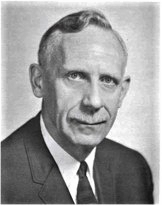
\includegraphics[width=\linewidth]{../figures/d2_bode_portrait.png}\end{minipage}\hfill
\begin{minipage}{.82\linewidth}\tiny H.\,W.\ Bode (1905--1982), Bell Labs. \credit{Unknown author, Public domain, via Wikimedia Commons}\end{minipage}
\column{.56\textwidth}
\centering
\begin{tikzpicture}
\begin{groupplot}[group style={group size=1 by 2,vertical sep=4mm,x descriptions at=edge bottom},
  mkplot,width=7.6cm,height=3.45cm,xmode=log,xmin=0.01,xmax=1000,log basis x=10]
\nextgroupplot[ylabel={$|G|$ [dB]},ymin=-30,ymax=70,ytick={-20,0,20,40,60},legend pos=north east,
  title={\scriptsize $G(s)=\dfrac{100(s+1)}{s(s+10)}$},title style={yshift=-1mm}]
  \addplot[mkBlue,very thick,domain=-2:3,samples=150] ({10^x},{20*log10(100)+10*log10(1+10^(2*x))-20*x-10*log10(100+10^(2*x))});
  \addlegendentry{exact}
  \addplot[mkOrange,thick,dashed] coordinates {(0.01,60)(1,20)(10,20)(1000,-20)}; \addlegendentry{asymptotes}
\nextgroupplot[ylabel={$\angle G$ [deg]},xlabel={$\omega$ [rad/s]},ymin=-100,ymax=0,ytick={-90,-45,0}]
  \addplot[mkBlue,very thick,domain=-2:3,samples=150] ({10^x},{-90+atan(10^x)-atan(10^x/10)});
  \addplot[mkOrange,thick,dashed] coordinates {(0.01,-90)(0.1,-90)(1,-45)(10,-45)(100,-90)(1000,-90)};
\end{groupplot}
\end{tikzpicture}\\
\scriptsize Low frequency: $G\approx10/s$ (40\,dB at 0.1\,rad/s); zero at 1, pole at 10\,rad/s.
\end{columns}
\end{frame}

% ---------------------------------------------------------------------
\begin{frame}{Second-order frequency response: resonance}
\begin{columns}[T]
\column{.57\textwidth}
\centering
\begin{tikzpicture}
\begin{groupplot}[group style={group size=1 by 2,vertical sep=4mm,x descriptions at=edge bottom},
  mkplot,width=8.0cm,height=3.9cm,xmode=log,xmin=0.1,xmax=10,
  cycle list={{mkRed,thick},{mkOrange,thick},{mkBlue,very thick},{mkMid,thick,dashed},{mkSky,thick,dotted}}]
\nextgroupplot[ylabel={$|G|$ [dB]},ymin=-40,ymax=22,legend pos=south west,legend columns=2]
  \addplot+[domain=-1:1,samples=300] ({10^x},{-10*log10((1-10^(2*x))^2+(2*0.05*10^x)^2)}); \addlegendentry{$\zeta=0.05$}
  \addplot+[domain=-1:1,samples=200] ({10^x},{-10*log10((1-10^(2*x))^2+(2*0.2*10^x)^2)}); \addlegendentry{$0.2$}
  \addplot+[domain=-1:1,samples=200] ({10^x},{-10*log10((1-10^(2*x))^2+(2*0.5*10^x)^2)}); \addlegendentry{$0.5$}
  \addplot+[domain=-1:1,samples=200] ({10^x},{-10*log10((1-10^(2*x))^2+(2*0.707*10^x)^2)}); \addlegendentry{$0.707$}
  \addplot+[domain=-1:1,samples=200] ({10^x},{-10*log10((1-10^(2*x))^2+(2*1*10^x)^2)}); \addlegendentry{$1$}
\nextgroupplot[ylabel={$\angle G$ [deg]},xlabel={$\omega/\omega_n$},ymin=-185,ymax=5,ytick={-180,-90,0}]
  \addplot+[domain=-1:1,samples=300] ({10^x},{-atan2(2*0.05*10^x,1-10^(2*x))});
  \addplot+[domain=-1:1,samples=200] ({10^x},{-atan2(2*0.2*10^x,1-10^(2*x))});
  \addplot+[domain=-1:1,samples=200] ({10^x},{-atan2(2*0.5*10^x,1-10^(2*x))});
  \addplot+[domain=-1:1,samples=200] ({10^x},{-atan2(2*0.707*10^x,1-10^(2*x))});
  \addplot+[domain=-1:1,samples=200] ({10^x},{-atan2(2*1*10^x,1-10^(2*x))});
\end{groupplot}
\end{tikzpicture}
\column{.41\textwidth}
\scriptsize
$G(j\omega)=\dfrac{1}{1-(\omega/\omega_n)^2+j2\zeta\,\omega/\omega_n}$
\begin{itemize}
  \item Asymptotes: 0\,dB, then $-40$\,dB/dec beyond $\omega_n$; phase $0\to-180^\circ$; at $\omega_n$: $-90^\circ$, $|G|=1/(2\zeta)$.
  \item Resonance peak for $\zeta<0.707$:
\end{itemize}
\begin{eqbox}
\[
M_r=\frac{1}{2\zeta\sqrt{1-\zeta^2}},\qquad\omega_r=\omega_n\sqrt{1-2\zeta^2}
\]
\end{eqbox}
\begin{itemize}
  \item $\zeta=0.05$: $M_r=10.0$ (+20\,dB) -- typical of a \hl{coupling or belt resonance}.
  \item Half-power bandwidth of the peak: $\Delta\omega\approx2\zeta\omega_n$ $\Rightarrow$ estimate $\zeta$ from a measured FRF.
\end{itemize}
\end{columns}
\end{frame}

% ---------------------------------------------------------------------
\begin{frame}{Excitation signals for frequency-response measurement}
\begin{columns}[T]
\column{.5\textwidth}
\centering
\begin{tikzpicture}
\begin{groupplot}[group style={group size=1 by 3,vertical sep=2.5mm,x descriptions at=edge bottom},
  mkplot,width=7.0cm,height=2.55cm,xmin=0,xmax=1,ymin=-1.4,ymax=1.4,ytick={-1,0,1},
  every axis title/.style={at={(0.01,0.98)},anchor=north west,font=\tiny\bfseries,fill=white,inner sep=1pt}]
\nextgroupplot[title={linear chirp 1$\to$40\,Hz}]
  \addplot[mkBlue,thin] table[x=t,y=chirp] {data/excitation.dat};
\nextgroupplot[title={PRBS (7-bit LFSR, 64 bit/s)}]
  \addplot[mkOrange,thin,const plot] table[x=t,y=prbs] {data/excitation.dat};
\nextgroupplot[title={stepped sine (3, 6, 12, 24\,Hz)},xlabel={time [s]}]
  \addplot[mkMid,thin] table[x=t,y=stepped] {data/excitation.dat};
\end{groupplot}
\end{tikzpicture}
\column{.48\textwidth}
\scriptsize
\begin{tabular}{@{}p{1.25cm}p{1.75cm}p{1.75cm}@{}}
\toprule
Signal & Pro & Con\\
\midrule
Stepped sine & best SNR per line, nonlinearity visible & slow\\
Chirp / sweep & fast, smooth, low crest factor & transient leakage; windowing\\
PRBS & flat spectrum to $\approx0.44f_{\mathrm{bit}}$, periodic $\Rightarrow$ no leakage & binary $\Rightarrow$ excites backlash/friction\\
Multisine & designed spectrum, periodic & crest factor design needed\\
\bottomrule
\end{tabular}\\[3pt]
\begin{itemize}
  \item Amplitude: large enough to dominate noise and \hl{break friction}, small enough to avoid saturation.
  \item Use \term{periodic} excitation and an integer number of periods to avoid leakage.
  \item Average several periods/blocks to reduce noise variance.
\end{itemize}
\end{columns}
\end{frame}

% ---------------------------------------------------------------------
\begin{frame}{FRF measurement in servo drives}
\begin{columns}[T]
\column{.6\textwidth}
\centering
\begin{tikzpicture}[node distance=6mm]
  \node[sum] (s1) {};
  \node[blk,right=of s1] (C) {$C(s)$\\speed PI};
  \node[sum,right=7mm of C] (s2) {};
  \node[blk,right=of s2] (G) {$G(s)$\\drive+mech.};
  \draw[sig] ($(s1.west)-(6mm,0)$) node[left,lbl]{$r$}--(s1);
  \draw[sig] (s1)--(C);
  \draw[sig] (C)--(s2) node[midway,above,lbl]{$u_c$};
  \draw[sig] (s2)--(G) node[midway,above,lbl]{$u$};
  \draw[sig] (G)--++(13mm,0) node[right,lbl]{$y$};
  \fill ($(G.east)+(6mm,0)$) circle (1pt);
  \draw[sig] ($(G.east)+(6mm,0)$)--++(0,-11mm) -| (s1) node[pos=.95,left,lbl]{$-$};
  \node[blko,above=6mm of s2,minimum width=14mm] (inj) {excitation $w$\\(chirp/PRBS)};
  \draw[sig,mkOrange] (inj)--(s2);
\end{tikzpicture}\\[1mm]
\scriptsize
\begin{tabular}{@{}lll@{}}
\toprule
Ratio of spectra & Gives & Remark\\
\midrule
$\hat G=\hat S_{wy}/\hat S_{wu}$ & plant $G$ & robust in closed loop\\
$\hat S_{wy}/\hat S_{ww}$ & process sensitivity $GS$ & \\
$-\hat S_{wu_c}/\hat S_{ww}$ & $T$ (input side) & \\
$\hat S_{uy}/\hat S_{uu}$ ($H_1$) & $G$ only if open loop & \hl{biased} in closed loop\\
\bottomrule
\end{tabular}
\column{.38\textwidth}
\centering
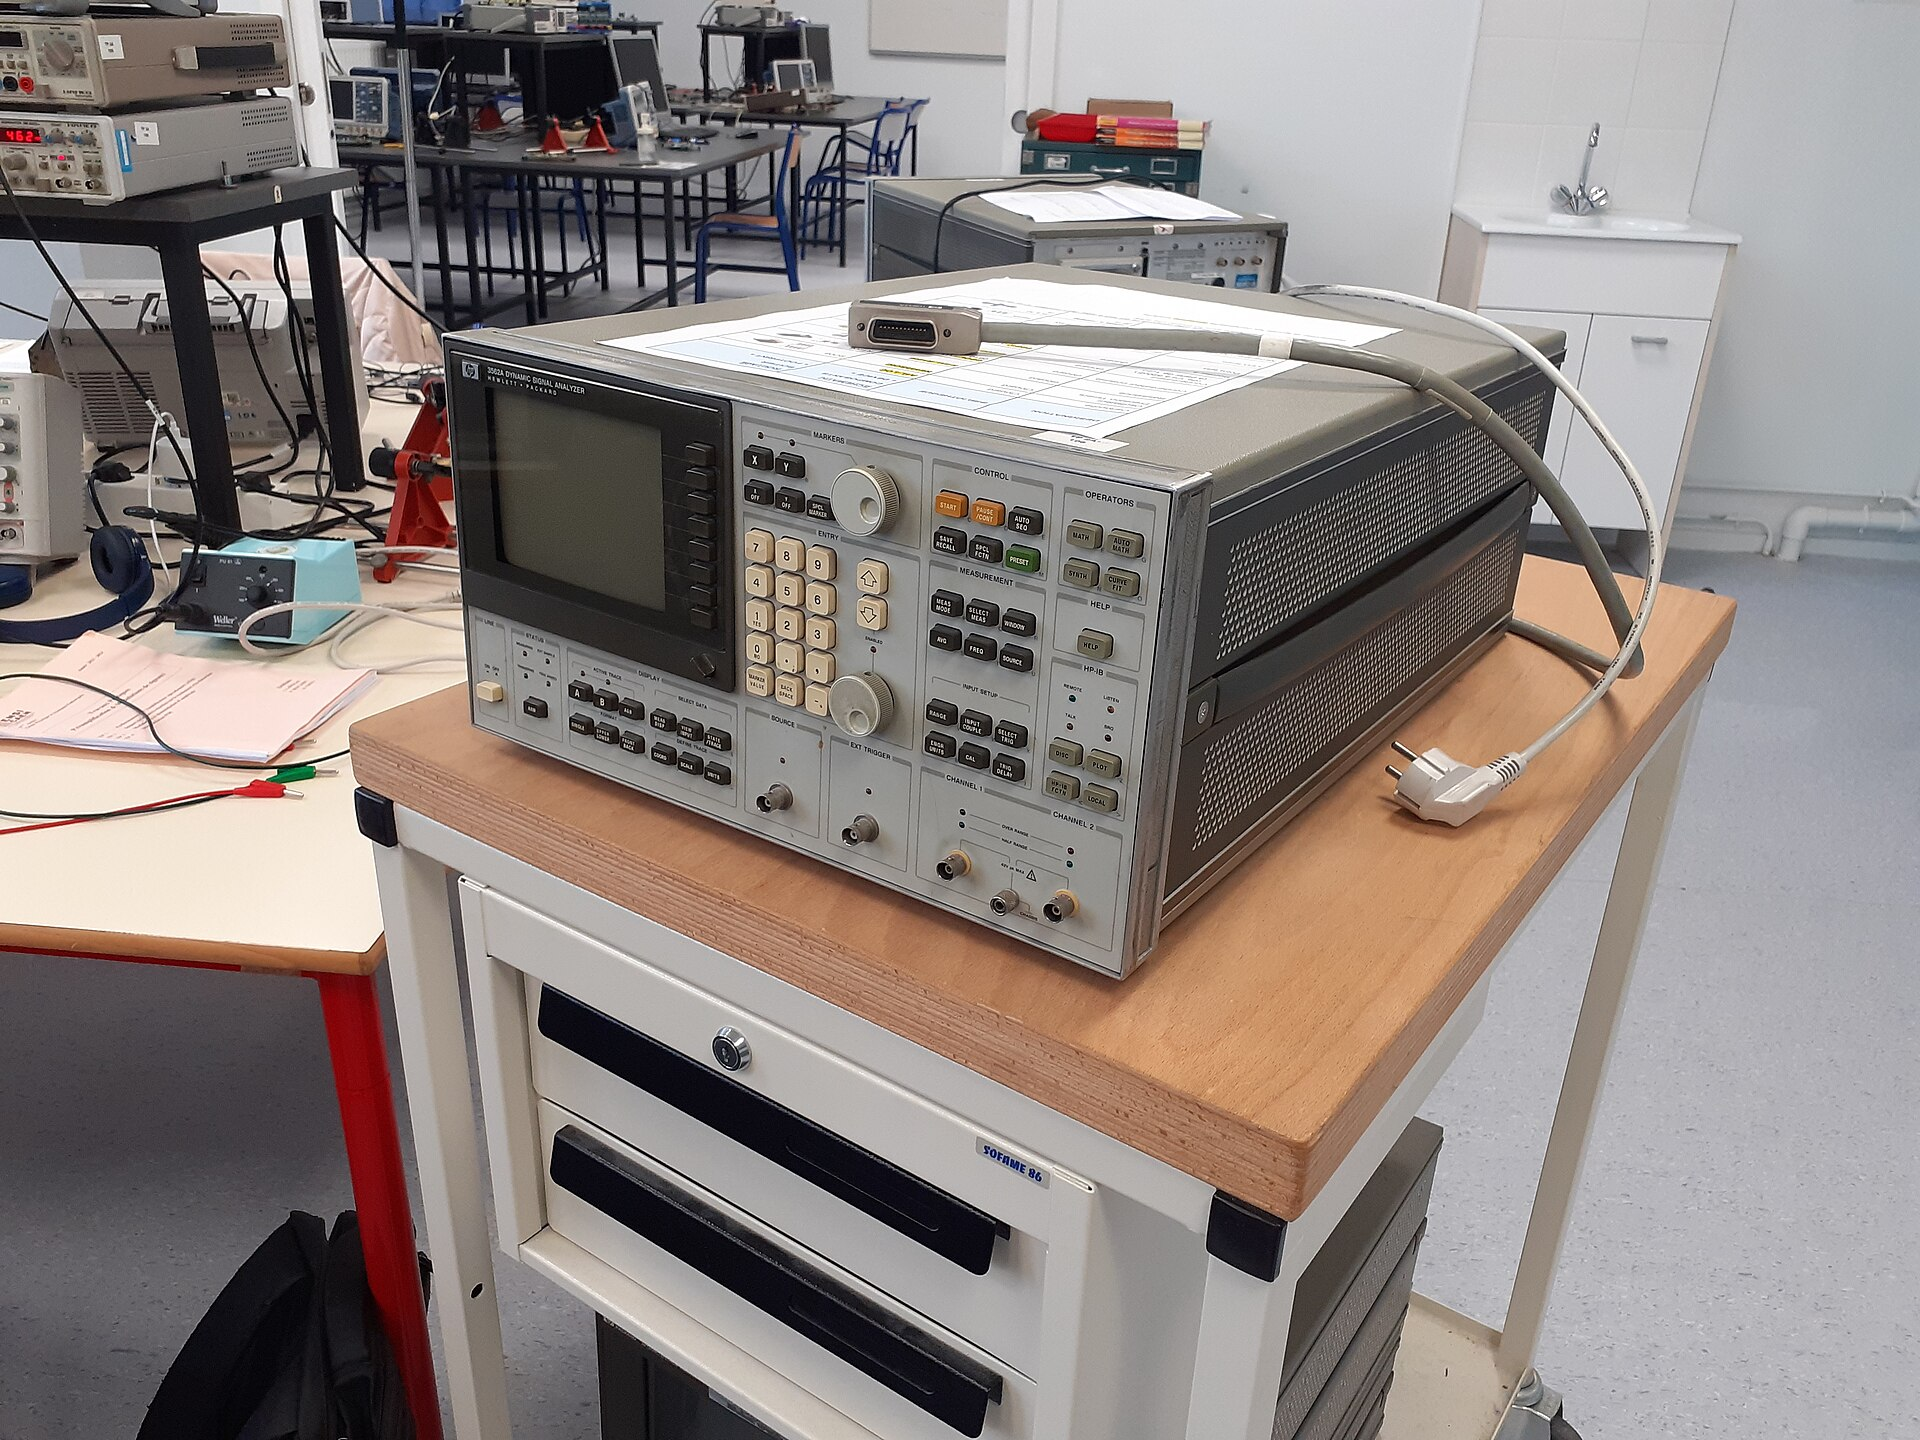
\includegraphics[width=\linewidth]{../figures/d2_signal_analyzer.jpg}\\
\credit{Loxyger, CC BY 4.0, via Wikimedia Commons}\\[1mm]
\scriptsize\raggedright
HP 3562A dynamic signal analyser (1985): the classic tool. Modern servo drives have the analyser \hl{built in}: the drive injects $w$ and records $u,y$ at the loop sample rate.\\[2pt]
Measure in \term{closed loop} (axis must hold position, gravity, safety) and compute $G$ from the cross-spectra with $w$.
\end{columns}
\end{frame}

% ---------------------------------------------------------------------
\begin{frame}{Measured FRF of a two-mass axis and coherence}
\begin{columns}[T]
\column{.56\textwidth}
\centering
\begin{tikzpicture}
\begin{groupplot}[group style={group size=1 by 2,vertical sep=4mm,x descriptions at=edge bottom},
  mkplot,width=8.0cm,height=3.7cm,xmode=log,xmin=1,xmax=1000]
\nextgroupplot[ylabel={$|\Omega_m/T_m|$ [dB]},ymin=-50,ymax=50,legend pos=south west]
  \addplot[mkBlue,very thick] table[x=f,y=mag] {data/twomass.dat}; \addlegendentry{two-mass}
  \addplot[mkOrange,thick,dashed] table[x=f,y=magrigid] {data/twomass.dat}; \addlegendentry{rigid $1/((J_m+J_l)s)$}
  \node[font=\tiny,anchor=north] at (axis cs:130,-22) {anti-res.};
  \node[font=\tiny,anchor=south] at (axis cs:260,30) {res.};
\nextgroupplot[ylabel={coherence $\gamma^2$},xlabel={frequency [Hz]},ymin=0,ymax=1.1,ytick={0,0.5,1}]
  \addplot[mkMid,very thick] table[x=f,y=coh] {data/twomass.dat};
\end{groupplot}
\end{tikzpicture}
\column{.42\textwidth}
\scriptsize
Motor inertia $J_m=2\times10^{-4}$, load $J_l=6\times10^{-4}$\,kg\,m$^2$, shaft stiffness $k=400$\,Nm/rad:
\begin{itemize}
  \item anti-resonance $f_{ar}=\frac{1}{2\pi}\sqrt{k/J_l}=130$\,Hz
  \item resonance $f_r=\frac{1}{2\pi}\sqrt{k\frac{J_m+J_l}{J_mJ_l}}=260$\,Hz \;($f_r/f_{ar}=\sqrt{1+J_l/J_m}=2$)
\end{itemize}
\begin{eqbox}
\[
\gamma^2(\omega)=\frac{|\hat S_{uy}|^2}{\hat S_{uu}\hat S_{yy}}\in[0,1]
\]
\end{eqbox}
\begin{itemize}
  \item $\gamma^2\approx1$: output linearly explained by input. Low $\gamma^2$: noise, nonlinearity, leakage.
  \item Coherence drops at the \hl{anti-resonance} (tiny output) and at high frequency $\Rightarrow$ trust $\hat G$ only where $\gamma^2\gtrsim0.8$.
\end{itemize}
\end{columns}
\end{frame}

% ---------------------------------------------------------------------
\begin{frame}{Model uncertainty}
\begin{columns}[T]
\column{.54\textwidth}
\centering
\begin{tikzpicture}
\begin{axis}[mkplot,width=7.8cm,height=5.4cm,xmode=log,xmin=1,xmax=1000,ymin=-50,ymax=30,
  xlabel={frequency [Hz]},ylabel={magnitude [dB]},legend pos=south west,legend cell align=left]
  \addplot[mkGray,very thick,name path=inv] table[x=f,y=invD] {data/uncertainty.dat}; \addlegendentry{$1/|\Delta|$ (allowed $|T|$)}
  \addplot[mkGreen,very thick] table[x=f,y=T30] {data/uncertainty.dat}; \addlegendentry{$|T|$, bandwidth 30\,Hz}
  \addplot[mkRed,very thick,dashed] table[x=f,y=T150] {data/uncertainty.dat}; \addlegendentry{$|T|$, bandwidth 150\,Hz}
  \path[name path=top] (axis cs:1,30)--(axis cs:1000,30);
  \addplot[mkGray,opacity=.12,forget plot] fill between[of=inv and top];
  \node[font=\tiny,mkRed,anchor=south] at (axis cs:300,5) {violation};
\end{axis}
\end{tikzpicture}
\column{.44\textwidth}
\scriptsize
Every model is wrong somewhere. Describe the error as a \term{multiplicative perturbation}:
\[
G_{\mathrm{true}}(s)=G_0(s)\big(1+\Delta(s)\big)
\]
Here $G_0$ = rigid-body model, $G_{\mathrm{true}}$ = two-mass system of the previous slide.
\begin{keybox}[Robust stability (small-gain)]
\scriptsize
If the nominal loop is stable, it stays stable for all $\Delta$ with $|\Delta(j\omega)|\le|W(j\omega)|$ iff
\[
|T(j\omega)|\,|W(j\omega)|<1\quad\forall\omega
\]
\end{keybox}
\begin{itemize}
  \item Relative error is small at low frequency and $>100\,\%$ near resonances.
  \item $\Rightarrow$ The bandwidth must stay \hl{below the first mechanical resonance} unless the resonance is modelled (notch filters, Day 3).
\end{itemize}
\end{columns}
\end{frame}

% ---------------------------------------------------------------------
\begin{frame}{Session 2.3 -- Summary}
\begin{keybox}[Key take-aways]
\begin{itemize}
  \item Combine physics (structure) with measurement (parameters): grey-box models are the servo engineer's default.
  \item Step tests give FOPDT ($K,\tau,\theta$) or 2nd-order ($\zeta,\omega_n$ from $M_p$, $t_p$) models quickly.
  \item The Bode diagram is built from asymptotes: $\pm20$\,dB/dec per real pole/zero, $-40$\,dB/dec and a peak $1/(2\zeta)$ per resonant pair.
  \item FRF measurement: periodic excitation (chirp, PRBS, multisine), averaging, cross-spectra with the injected signal in closed loop.
  \item Check \hl{coherence}; quantify model error $\Delta(j\omega)$ -- it limits the achievable bandwidth.
\end{itemize}
\end{keybox}
\end{frame}

% =====================================================================
\section{2.4 PID and Basic Control Structures}
% =====================================================================

\begin{frame}{The standard feedback loop}
\begin{columns}[T]
\column{.66\textwidth}
\centering
\begin{tikzpicture}[node distance=7mm]
  \node[sum] (s1) {};
  \node[blk,right=of s1] (C) {$C(s)$};
  \node[sum,right=of C] (s2) {};
  \node[blk,right=of s2] (G) {$G(s)$};
  \node[sum,right=8mm of G] (s3) {};
  \draw[sig] ($(s1.west)-(8mm,0)$) node[left,lbl]{$r$}--(s1) node[pos=.7,above,lbl]{$+$};
  \draw[sig] (s1)--(C) node[midway,above,lbl]{$e$};
  \draw[sig] (C)--(s2) node[midway,above,lbl]{$u$};
  \draw[sig] (s2)--(G);
  \draw[sig] (G)--(s3);
  \draw[sig] (s3)--++(12mm,0) node[right,lbl]{$y$};
  \draw[sig] ($(s2.north)+(0,7mm)$) node[above,lbl]{$d$ (load)}--(s2);
  \draw[sig] ($(s3.north)+(0,7mm)$) node[above,lbl]{$d_o$}--(s3);
  \node[sum,below=8mm of s3] (s4) {};
  \fill ($(s3.east)+(5mm,0)$) circle (1pt);
  \draw[sig] ($(s3.east)+(5mm,0)$) |- (s4);
  \draw[sig] ($(s4.east)+(8mm,0)$) node[right,lbl]{$n$}--(s4);
  \draw[sig] (s4) -| (s1) node[pos=.95,left,lbl]{$-$};
\end{tikzpicture}\\[2mm]
\begin{eqbox}
\footnotesize
\[
Y=\underbrace{\frac{L}{1+L}}_{T}R+\underbrace{\frac{G}{1+L}}_{GS}D+\underbrace{\frac{1}{1+L}}_{S}D_o-T\,N
\]
\end{eqbox}
\scriptsize
\begin{itemize}
  \item Large $|L|$ $\Rightarrow$ $S\to0$: disturbances rejected, $y$ follows $r$ -- \hl{but} $T\to1$: noise passes to $y$.
  \item Four ``gang of four'' transfer functions $S$, $T$, $GS$, $CS$ must \emph{all} be stable [\AA str\"om \& Murray, 2008].
\end{itemize}
\column{.32\textwidth}
\centering
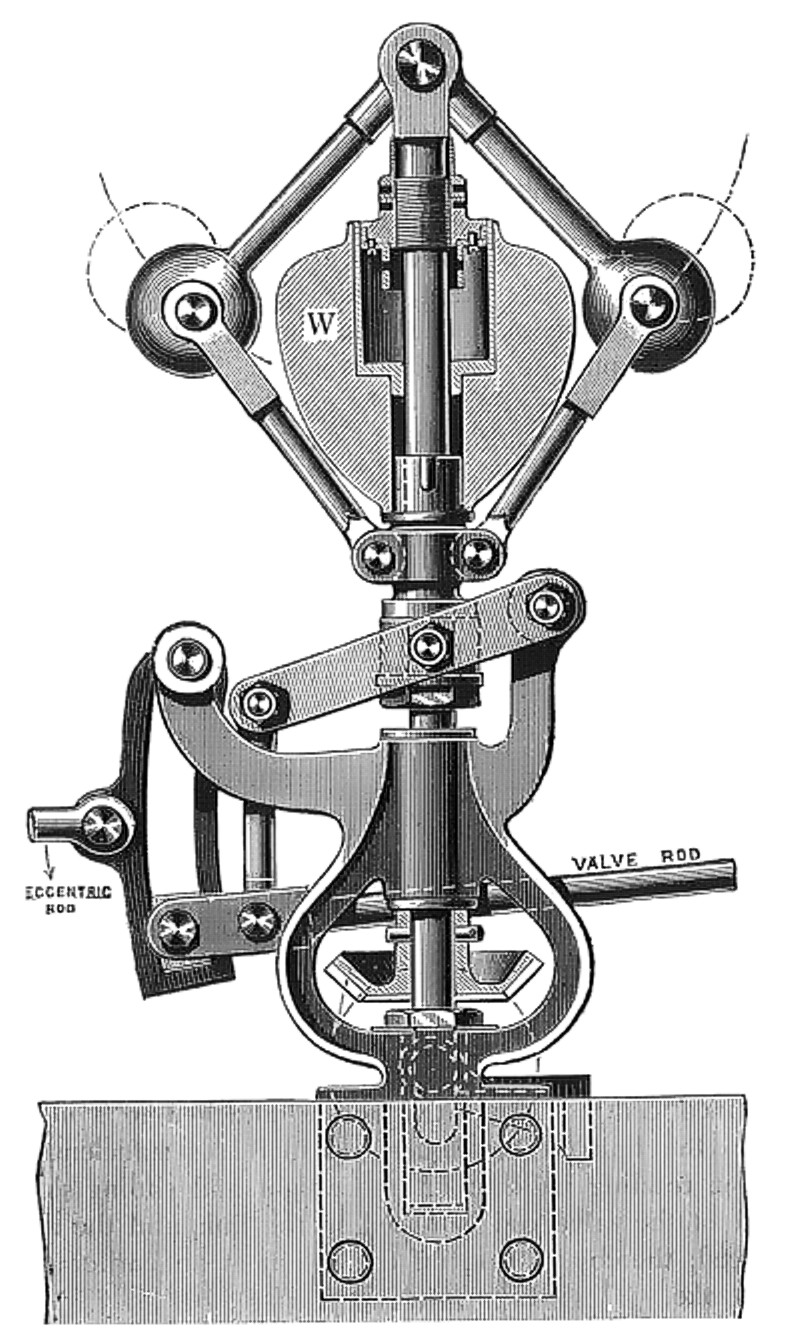
\includegraphics[height=3.4cm]{../figures/d2_governor.jpg}\\
\credit{Heat Engines (1913), scan by Andy Dingley, Public domain, via Wikimedia Commons}\\[1mm]
\scriptsize\raggedright
Watt's centrifugal governor: a mechanical \term{proportional} speed controller; Maxwell's 1868 analysis ``On Governors'' started control theory.
\end{columns}
\end{frame}

% ---------------------------------------------------------------------
\begin{frame}{Effects of P, I and D actions}
\begin{columns}[T]
\column{.5\textwidth}
\centering
\begin{tikzpicture}
\begin{axis}[mkplot,width=6.9cm,height=4.5cm,xlabel={time [s]},ylabel={$y$},xmin=0,xmax=20,ymin=0,ymax=1.6,
  title={\scriptsize P only, $G=1/(s+1)^3$},title style={yshift=-1.5mm},legend pos=north east,legend columns=2]
  \addplot[mkSky,thick] table[x=t,y=k05] {data/p_control.dat}; \addlegendentry{$K_p=0.5$}
  \addplot[mkMid,thick] table[x=t,y=k1] {data/p_control.dat}; \addlegendentry{$1$}
  \addplot[mkBlue,very thick] table[x=t,y=k2] {data/p_control.dat}; \addlegendentry{$2$}
  \addplot[mkOrange,thick] table[x=t,y=k4] {data/p_control.dat}; \addlegendentry{$4$}
\end{axis}
\end{tikzpicture}\\
\scriptsize Offset $e_\infty=1/(1+K_p)$; $K_p=8$ $\Rightarrow$ sustained oscillation.
\column{.5\textwidth}
\centering
\begin{tikzpicture}
\begin{axis}[mkplot,width=6.9cm,height=4.5cm,xlabel={time [s]},xmin=0,xmax=20,ymin=0,ymax=1.6,
  title={\scriptsize same plant, four controllers},title style={yshift=-1.5mm},legend pos=north east,legend columns=2]
  \addplot[mkSky,thick] table[x=t,y=P] {data/pid_compare.dat}; \addlegendentry{P}
  \addplot[mkMid,thick,dashed] table[x=t,y=PD] {data/pid_compare.dat}; \addlegendentry{PD}
  \addplot[mkOrange,thick] table[x=t,y=PI] {data/pid_compare.dat}; \addlegendentry{PI}
  \addplot[mkBlue,very thick] table[x=t,y=PID] {data/pid_compare.dat}; \addlegendentry{PID}
\end{axis}
\end{tikzpicture}\\
\scriptsize P: $K_p\!=\!1$; PI: $K_p\!=\!1,T_i\!=\!2$; PD: $K_p\!=\!1,T_d\!=\!0.8$; PID: $K_p\!=\!2,T_i\!=\!2,T_d\!=\!0.6$ ($N\!=\!10$).
\end{columns}
\vspace{1mm}
\scriptsize
\begin{tabular}{@{}lllll@{}}
\toprule
Increase \ldots & rise time & overshoot & steady-state error & stability margin\\
\midrule
$K_p$ & faster & larger & smaller (not zero) & lower\\
$1/T_i$ (I action) & faster & larger & \hl{eliminated} (step) & lower (phase lag)\\
$T_d$ (D action) & little change & smaller & no effect & higher (phase lead), but noise $\uparrow$\\
\bottomrule
\end{tabular}
\end{frame}

% ---------------------------------------------------------------------
\begin{frame}{PID forms: parallel, ideal (ISA) and series}
\begin{columns}[T]
\column{.62\textwidth}
\scriptsize
\begin{tabular}{@{}lll@{}}
\toprule
Form & Transfer function & Typical use\\
\midrule
Parallel & $C=K_p+\dfrac{K_i}{s}+K_ds$ & textbooks, drives\\[6pt]
Ideal (ISA) & $C=K_p\Big(1+\dfrac{1}{T_is}+T_ds\Big)$ & process controllers\\[6pt]
Series (interacting) & $C=K_p'\Big(1+\dfrac{1}{T_i's}\Big)\big(1+T_d's\big)$ & legacy, PLCs\\
\bottomrule
\end{tabular}\\[4pt]
\textbf{Conversions:} $K_i=K_p/T_i$, $K_d=K_pT_d$; series $\to$ ideal:
\[
K_p=K_p'\frac{T_i'+T_d'}{T_i'},\quad T_i=T_i'+T_d',\quad T_d=\frac{T_i'T_d'}{T_i'+T_d'}
\]
\begin{itemize}
  \item The series form always has real zeros (possible only if $T_i\ge4T_d$ in ideal form).
  \item Changing $K_p$ in the ideal form scales all three actions; in the parallel form only P.
  \item \hl{Pitfall}: copying gains between devices without checking the form and units (s vs.\ min, \% vs.\ engineering units, rad vs.\ rev).
\end{itemize}
\column{.36\textwidth}
\centering
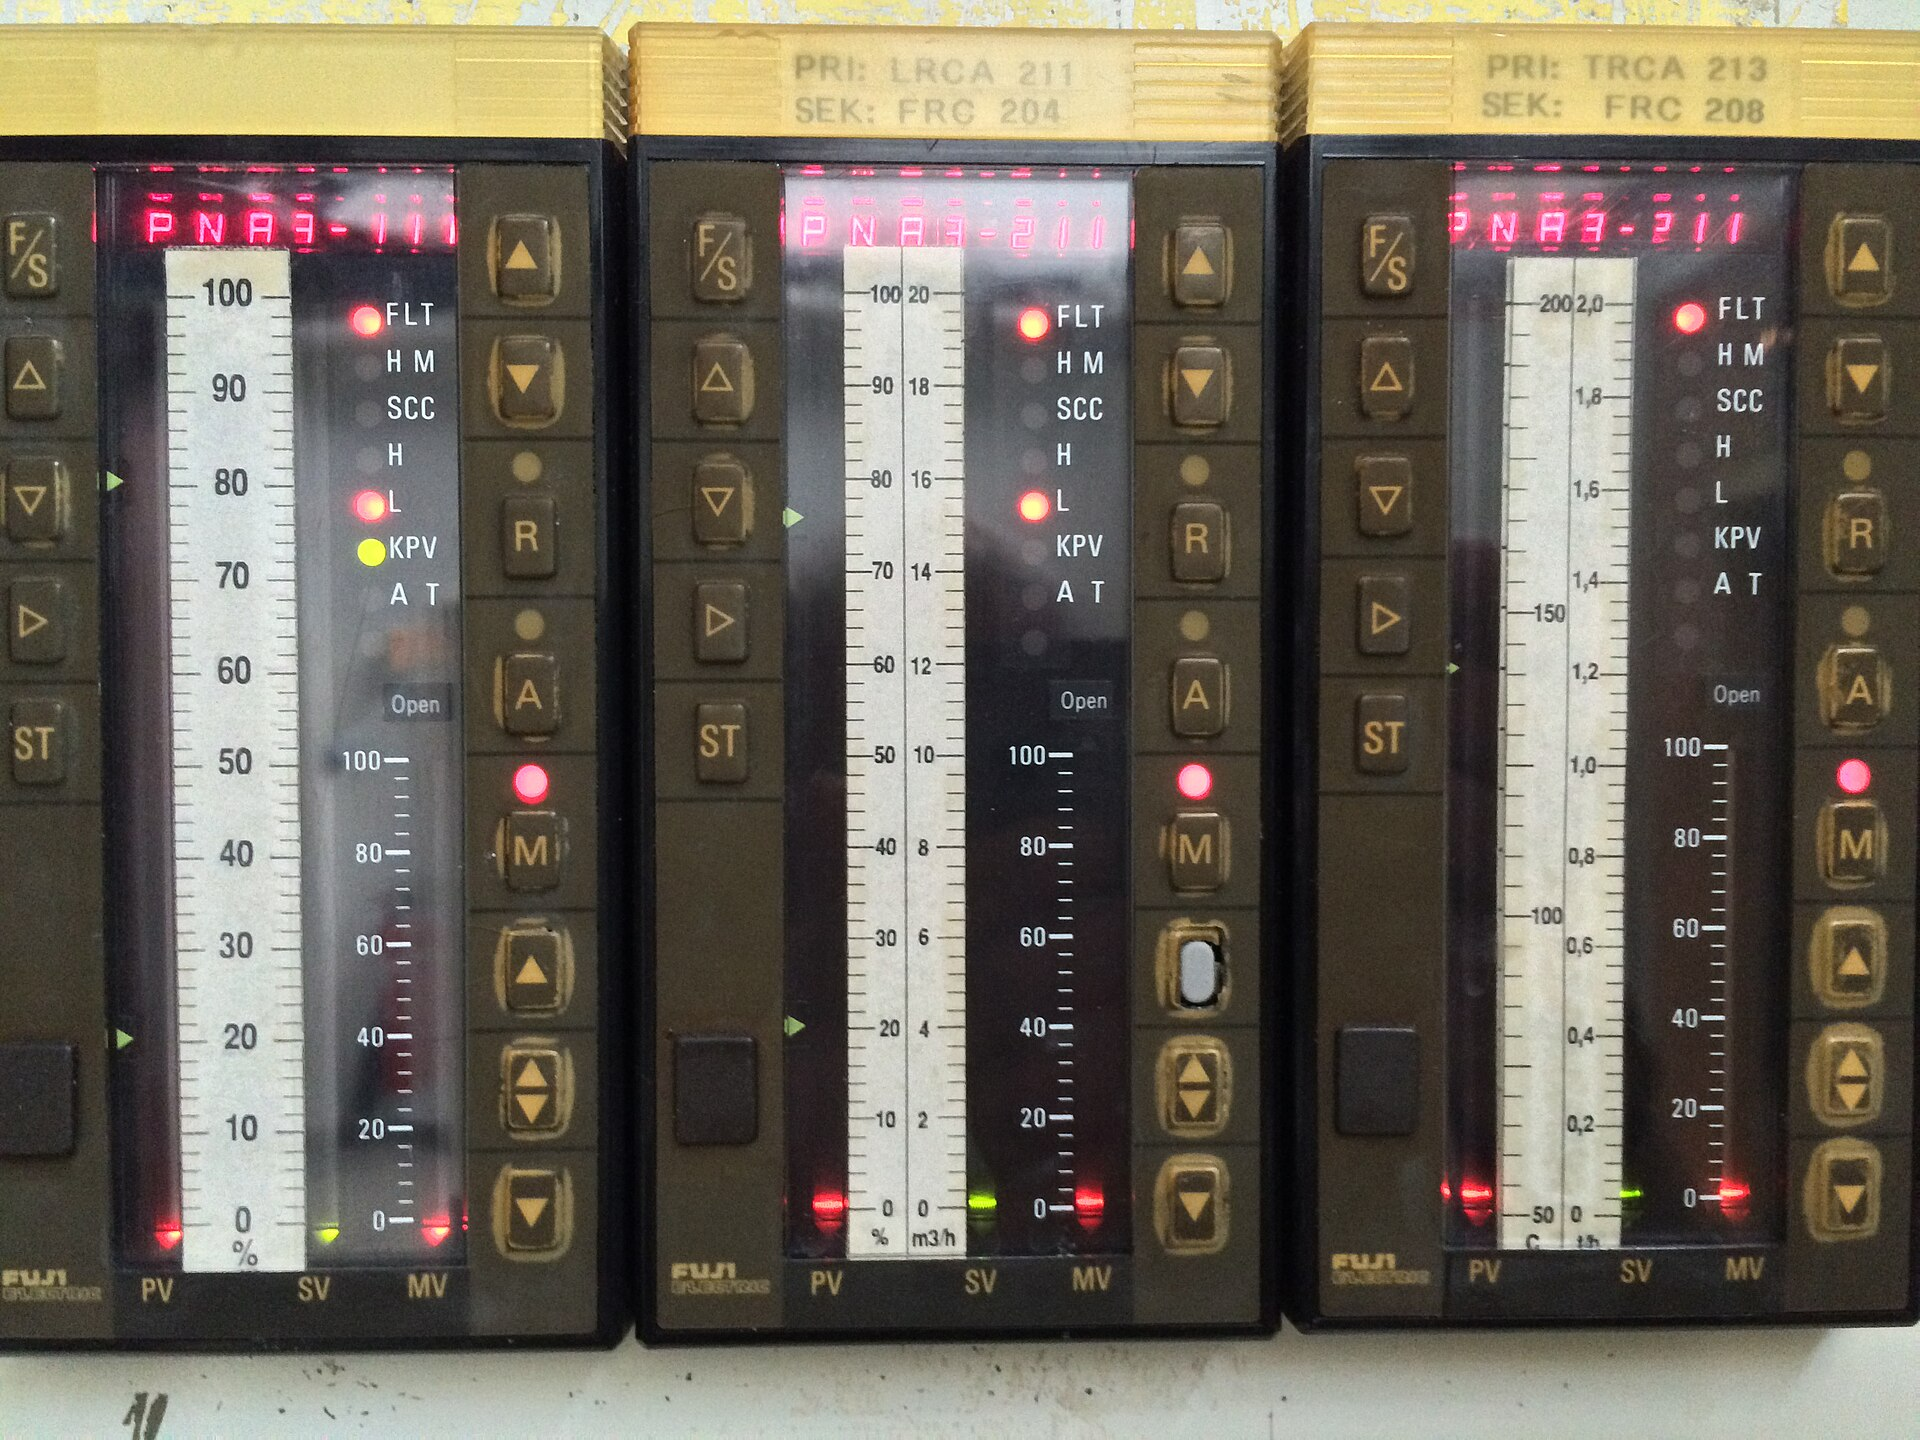
\includegraphics[width=\linewidth]{../figures/d2_pid_controllers.jpg}\\
\credit{Bitjungle, CC BY-SA 4.0, via Wikimedia Commons}\\[1mm]
\scriptsize\raggedright
Industrial PID controllers: tuning parameters are usually entered as $K_p$ (or proportional band $100/K_p$\,\%), $T_i$, $T_d$ in the ideal form.
\end{columns}
\end{frame}

% ---------------------------------------------------------------------
\begin{frame}{Classical tuning: Ziegler--Nichols (1942)}
\begin{columns}[T]
\column{.5\textwidth}
\scriptsize
\textbf{Ultimate-sensitivity method:} P-only, raise $K_p$ until sustained oscillation: ultimate gain $K_u$, period $T_u$.
\begin{center}
\begin{tabular}{@{}lccc@{}}
\toprule
 & $K_p$ & $T_i$ & $T_d$\\
\midrule
P & $0.5K_u$ & -- & --\\
PI & $0.45K_u$ & $T_u/1.2$ & --\\
PID & $0.6K_u$ & $T_u/2$ & $T_u/8$\\
\bottomrule
\end{tabular}
\end{center}
\textbf{Step-response method:} FOPDT $(K,\tau,\theta)$, $a=K\theta/\tau$.
\begin{center}
\begin{tabular}{@{}lccc@{}}
\toprule
 & $K_p$ & $T_i$ & $T_d$\\
\midrule
P & $1/a$ & -- & --\\
PI & $0.9/a$ & $3\theta$ & --\\
PID & $1.2/a$ & $2\theta$ & $\theta/2$\\
\bottomrule
\end{tabular}
\end{center}
\column{.48\textwidth}
\begin{defbox}[Worked example]
\scriptsize
Plant $G=1/(s+1)^3$. Phase $-180^\circ$ when $3\arctan\omega=180^\circ$ $\Rightarrow$ $\omega_u=\sqrt3$ rad/s;
$|G(j\omega_u)|=1/8$ $\Rightarrow$ $K_u=8$, $T_u=2\pi/\sqrt3=3.63$\,s.\\
ZN PID: $K_p=4.8$, $T_i=1.81$\,s, $T_d=0.45$\,s.
\end{defbox}
\begin{keybox}[Critique]
\scriptsize
\begin{itemize}
  \item Designed for \hl{quarter-amplitude decay} ($\zeta\approx0.2$): aggressive, $M_s$ often $>3$.
  \item Pushing a real machine to the stability limit can be unsafe.
  \item Use ZN only as a starting point; modern rules (SIMC, AMIGO, lambda) are more robust [\AA str\"om \& H\"agglund, 2006].
\end{itemize}
\end{keybox}
\end{columns}
\end{frame}

% ---------------------------------------------------------------------
\begin{frame}{Model-based tuning: lambda, SIMC, Cohen--Coon}
\begin{columns}[T]
\column{.52\textwidth}
\scriptsize
For FOPDT $G=Ke^{-\theta s}/(\tau s+1)$, PI controller $K_p(1+1/(T_is))$:\\[2pt]
\begin{tabular}{@{}lll@{}}
\toprule
Method & $K_p$ & $T_i$\\
\midrule
Lambda (IMC) & $\dfrac{\tau}{K(\lambda+\theta)}$ & $\tau$\\[6pt]
SIMC [Skogestad 2003] & $\dfrac{\tau}{K(\tau_c+\theta)}$ & $\min\{\tau,\,4(\tau_c+\theta)\}$\\[6pt]
Cohen--Coon & $\dfrac{\tau}{K\theta}\Big(0.9+\dfrac{\theta}{12\tau}\Big)$ & $\theta\dfrac{30+3\theta/\tau}{9+20\theta/\tau}$\\
\bottomrule
\end{tabular}\\[4pt]
\begin{itemize}
  \item One intuitive knob: the desired closed-loop time constant $\lambda$ or $\tau_c$.
  \item SIMC default $\tau_c=\theta$: good trade-off, $M_s\approx1.6$--$1.7$.
  \item Lambda tuning: $T_i=\tau$ cancels the plant pole $\Rightarrow$ slow load-disturbance recovery if $\tau\gg\theta$.
\end{itemize}
\column{.46\textwidth}
\begin{defbox}[Example: FOPDT of session 2.3]
\scriptsize
$K=2$, $\tau=1.29$\,s, $\theta=0.57$\,s ($\theta/\tau=0.44$)\\[3pt]
\begin{tabular}{@{}lcc@{}}
\toprule
Rule & $K_p$ & $T_i$ [s]\\
\midrule
ZN step (PI) & 1.02 & 1.71\\
Cohen--Coon (PI) & 1.06 & 1.00\\
SIMC, $\tau_c=\theta$ & 0.56 & 1.29\\
Lambda, $\lambda=\tau$ & 0.35 & 1.29\\
\bottomrule
\end{tabular}\\[3pt]
Spread of almost 3:1 in $K_p$ -- the rules encode \hl{different robustness targets}, not ``the'' answer.
\end{defbox}
\begin{notebox}
\scriptsize
Servo drives typically use model-based rules from inertia and bandwidth instead (see cascade slide).
\end{notebox}
\end{columns}
\end{frame}

% ---------------------------------------------------------------------
\begin{frame}{Loop shaping: designing $|L(j\omega)|$ directly}
\begin{columns}[T]
\column{.55\textwidth}
\centering
\begin{tikzpicture}
\begin{axis}[mkplot,width=7.8cm,height=5.6cm,xmode=log,xmin=0.01,xmax=100,ymin=-60,ymax=70,
  xlabel={$\omega/\omega_c$},ylabel={$|L(j\omega)|$ [dB]}]
  \fill[mkGreen,opacity=.15] (axis cs:0.01,-60) rectangle (axis cs:0.08,20);
  \fill[mkRed,opacity=.15] (axis cs:8,-20) rectangle (axis cs:100,70);
  \addplot[mkBlue,very thick,domain=-2:2,samples=200] ({10^x},{-20*x+10*log10(1+(0.2/10^x)^2)-20*log10(1+(10^x/5)^2)});
  \addplot[mkGray,dashed,domain=-2:2] ({10^x},{0});
  \node[font=\tiny,mkGreen,align=center] at (axis cs:0.028,-40) {performance:\\$|L|\gg1$\\(tracking,\\disturbance\\rejection)};
  \node[font=\tiny,mkRed,align=center] at (axis cs:28,40) {robustness:\\$|L|\ll1$\\(noise,\\unmodelled\\dynamics)};
  \node[font=\tiny,mkNavy,anchor=south west] at (axis cs:1.1,2) {crossover, slope $\approx-20$\,dB/dec};
  \fill[mkOrange] (axis cs:1,0) circle (1.8pt);
\end{axis}
\end{tikzpicture}
\column{.43\textwidth}
\scriptsize
Since $S=1/(1+L)$ and $T=L/(1+L)$:
\begin{itemize}
  \item $|L|\gg1$ $\Rightarrow$ $|S|\approx1/|L|$ small: good tracking and load rejection.
  \item $|L|\ll1$ $\Rightarrow$ $|T|\approx|L|$ small: noise and model errors suppressed.
  \item Around $\omega_c$: slope about $-20$\,dB/dec over about a decade $\Rightarrow$ phase near $-90^\circ\ldots-130^\circ$ $\Rightarrow$ healthy PM (Bode gain--phase relation).
\end{itemize}
\begin{keybox}[Loop-shaping with PID]
\scriptsize
I action raises low-frequency gain (slope $-40$\,dB/dec below $1/T_i$);
D action adds phase lead around $\omega_c$; the filter $N$ and extra low-pass filters give high-frequency roll-off.
Practical rule: $1/T_i\approx\omega_c/4\ldots\omega_c/10$.
\end{keybox}
\end{columns}
\end{frame}

% ---------------------------------------------------------------------
\begin{frame}{Derivative action: filtering and placement}
\begin{columns}[T]
\column{.5\textwidth}
\centering
\begin{tikzpicture}
\begin{axis}[mkplot,width=7.0cm,height=5.0cm,xmode=log,xmin=0.01,xmax=1000,ymin=-30,ymax=50,
  xlabel={$\omega T_d$},ylabel={gain of D-part [dB]},legend pos=north west]
  \addplot[mkRed,thick,dashed,domain=-2:3,samples=100] ({10^x},{20*x}); \addlegendentry{ideal $K_pT_ds$}
  \addplot[mkBlue,very thick,domain=-2:3,samples=150] ({10^x},{20*x-10*log10(1+(10^x/10)^2)}); \addlegendentry{filtered, $N=10$}
  \addplot[mkOrange,thick,domain=-2:3,samples=150] ({10^x},{20*x-10*log10(1+(10^x/5)^2)}); \addlegendentry{filtered, $N=5$}
  \node[font=\tiny,anchor=west] at (axis cs:15,26) {limit $20\log N$};
\end{axis}
\end{tikzpicture}
\column{.48\textwidth}
\scriptsize
An ideal differentiator has unbounded high-frequency gain: encoder quantisation and noise are amplified.
\begin{eqbox}
\[
C(s)=K_p\Big(1+\frac{1}{T_is}+\frac{T_ds}{1+T_ds/N}\Big),\quad N\approx5\ldots20
\]
\end{eqbox}
\begin{itemize}
  \item High-frequency D-gain limited to $K_pN$; filter pole at $N/T_d$.
  \item Alternatively filter the measurement: $C(s)\cdot\frac{1}{(T_fs+1)^2}$ (2nd-order roll-off).
  \item \hl{Derivative on measurement}, $u_D=-K_pT_d\,\dot y_f$: avoids the ``derivative kick'' at set-point steps.
  \item Servo practice: D-action on position = velocity feedback from the encoder; in cascade form this is the inner velocity loop.
  \item Example: 20-bit encoder, $T_s=125\,\mu$s: one count $\Rightarrow$ velocity step of $2\pi/(2^{20}T_s)=0.048$\,rad/s per sample.
\end{itemize}
\end{columns}
\end{frame}

% ---------------------------------------------------------------------
\begin{frame}{Set-point weighting: two degrees of freedom}
\begin{columns}[T]
\column{.5\textwidth}
\centering
\begin{tikzpicture}
\begin{axis}[mkplot,width=7.0cm,height=5.0cm,xlabel={time [s]},ylabel={$y$},xmin=0,xmax=20,ymin=0,ymax=1.45,legend pos=south east]
  \addplot[mkRed,thick] table[x=t,y=b1] {data/spweight.dat}; \addlegendentry{$b=1$ (error feedback)}
  \addplot[mkOrange,thick,dashed] table[x=t,y=b05] {data/spweight.dat}; \addlegendentry{$b=0.5$}
  \addplot[mkBlue,very thick] table[x=t,y=b0] {data/spweight.dat}; \addlegendentry{$b=0$ (I-P)}
\end{axis}
\end{tikzpicture}\\
\scriptsize PI, $K_p=2$, $T_i=2.5$\,s, $G=1/(s+1)^3$. Overshoot: 33\,\%, 3.4\,\%, 0.3\,\%.
\column{.48\textwidth}
\scriptsize
Weight the set-point differently in each term:
\begin{eqbox}
\[
u=K_p\Big[(b\,r-y)+\frac1{T_i}\!\int(r-y)\,dt+T_d\frac{d}{dt}(c\,r-y_f)\Big]
\]
\end{eqbox}
\begin{itemize}
  \item The I-term must use the true error ($r-y$) so the steady state is exact.
  \item Typical: $c=0$ (no derivative kick), $0\le b\le1$.
  \item Feedback properties ($L$, $S$, $T$, margins, \hl{load-disturbance response}) are \emph{unchanged}: $b,c$ only shape the set-point response.
  \item Tune $K_p,T_i,T_d$ for disturbances and robustness first, then $b$ for the set-point.
  \item Same idea in servos: reference pre-filter or trajectory generator + feedforward.
\end{itemize}
\end{columns}
\end{frame}

% ---------------------------------------------------------------------
\begin{frame}{Actuator saturation and integrator windup}
\begin{columns}[T]
\column{.58\textwidth}
\centering
\begin{tikzpicture}
\begin{groupplot}[group style={group size=1 by 2,vertical sep=3mm,x descriptions at=edge bottom},
  mkplot,width=8.2cm,height=3.7cm,xmin=0,xmax=12]
\nextgroupplot[ylabel={output $y$},ymin=0,ymax=1.3,legend pos=south east,legend columns=3]
  \addplot[mkRed,thick] table[x=t,y=ynone] {data/windup.dat}; \addlegendentry{no anti-windup}
  \addplot[mkOrange,thick,dashed] table[x=t,y=yclamp] {data/windup.dat}; \addlegendentry{clamping}
  \addplot[mkBlue,very thick,dotted] table[x=t,y=ybc] {data/windup.dat}; \addlegendentry{back-calc.}
\nextgroupplot[ylabel={$u$, $v$},xlabel={time [s]},ymin=-2,ymax=4.5]
  \addplot[mkSky,thin] table[x=t,y=vnone] {data/windup.dat};
  \addplot[mkRed,thick] table[x=t,y=unone] {data/windup.dat};
  \addplot[mkOrange,thick,dashed] table[x=t,y=uclamp] {data/windup.dat};
  \addplot[mkBlue,very thick,dotted] table[x=t,y=ubc] {data/windup.dat};
  \addplot[mkGray,dashed,domain=0:12] {1.2};\addplot[mkGray,dashed,domain=0:12] {-1.2};
  \node[font=\tiny,mkSky,anchor=west] at (axis cs:2.5,3.3) {unsaturated controller output $v$ (no AW)};
\end{groupplot}
\end{tikzpicture}
\column{.40\textwidth}
\scriptsize
Plant $1/(s+1)$, PI $K_p=4$, $T_i=0.8$\,s, limit $|u|\le1.2$. Set-point $1\to0.4$ at 6\,s, load step at 9\,s.
\begin{itemize}
  \item While $u$ is saturated the loop is \hl{open}: the integrator keeps integrating the error.
  \item The ``wound-up'' integrator must be unwound by an error of opposite sign $\Rightarrow$ 18\,\% overshoot, long settling, sluggish reaction to the set-point change.
  \item In servos: current limit (torque), voltage limit (DC-link), speed limit in the cascade.
  \item Every saturating integrator needs anti-windup -- including the speed loop when the current reference is clamped.
\end{itemize}
\end{columns}
\end{frame}

% ---------------------------------------------------------------------
\begin{frame}{Anti-windup schemes}
\begin{columns}[T]
\column{.5\textwidth}
\centering
\textbf{\scriptsize Back-calculation (tracking)}\\[1mm]
\begin{tikzpicture}[node distance=5mm,font=\scriptsize]
  \node[blk,minimum width=8mm] (kp) {$K_p$};
  \node[blk,below=4mm of kp,minimum width=8mm] (ki) {$\frac{K_p}{T_i}$};
  \node[sum,right=of ki] (si) {};
  \node[blko,right=of si,minimum width=7mm] (int) {$\frac1s$};
  \node[sum,right=7mm of int] (sv) {};
  \node[blk,right=of sv,minimum width=11mm] (sat) {\tikz{\draw[thick](0,0)--(.12,0)--(.36,.24)--(.48,.24);}};
  \node[sum,below=6mm of sat] (se) {};
  \node[blk,left=7mm of se,minimum width=8mm] (tt) {$\frac1{T_t}$};
  \coordinate (in) at ($(kp.west)-(6mm,0)$);
  \draw[sig] ($(in)-(4mm,0)$) node[left]{$e$}--(kp);
  \draw[sig] (in) |- (ki); \fill (in) circle (1pt);
  \draw[sig] (ki)--(si); \draw[sig] (si)--(int); \draw[sig] (int)--(sv);
  \draw[sig] (kp) -| (sv);
  \draw[sig] (sv)--(sat) node[midway,above]{$v$};
  \draw[sig] (sat)--++(11mm,0) node[right]{$u$};
  \fill ($(sat.east)+(5mm,0)$) circle (1pt);
  \draw[sig] ($(sat.east)+(5mm,0)$) |- (se) node[pos=.9,above]{$+$};
  \fill ($(sv.east)+(2.5mm,0)$) circle (1pt);
  \draw[sig] ($(sv.east)+(2.5mm,0)$) |- (se.west) node[pos=.9,above]{$-$};
  \draw[sig] (se.south) |- ++(-1,-.3) -| (tt.south);
  \draw[sig] (tt) -| (si);
\end{tikzpicture}\\[1mm]
\scriptsize\raggedright
Integrator input: $\dfrac{K_p}{T_i}e+\dfrac{1}{T_t}(u-v)$. When saturated, the integrator is driven so that $v$ tracks $u$.
Choice: $T_t\approx\sqrt{T_iT_d}$, or $T_t\approx T_i/2$ for PI [\AA str\"om \& H\"agglund, 2006]. With a model of the limit, also works for rate limits.
\column{.48\textwidth}
\centering
\textbf{\scriptsize Conditional integration (clamping)}\\[1mm]
\begin{tikzpicture}[node distance=5mm,font=\scriptsize]
  \node[blk,minimum width=8mm] (kp) {$K_p$};
  \node[blk,below=4mm of kp,minimum width=8mm] (ki) {$\frac{K_p}{T_i}$};
  \node[right=4mm of ki,inner sep=0] (sw) {\tikz{\draw[thick,mkOrange](0,0)--(.35,.15);\fill(0,0)circle(1pt);\fill(.4,0)circle(1pt);}};
  \node[blko,right=4mm of sw,minimum width=7mm] (int) {$\frac1s$};
  \node[sum,right=6mm of int] (sv) {};
  \node[blk,right=of sv,minimum width=11mm] (sat) {\tikz{\draw[thick](0,0)--(.12,0)--(.36,.24)--(.48,.24);}};
  \node[blk,below=4mm of int,font=\tiny,align=center] (lg) {sat.\ \& $\operatorname{sgn}e=\operatorname{sgn}v$\\$\Rightarrow$ open};
  \coordinate (in) at ($(kp.west)-(6mm,0)$);
  \draw[sig] ($(in)-(4mm,0)$) node[left]{$e$}--(kp);
  \draw[sig] (in) |- (ki); \fill (in) circle (1pt);
  \draw[sig] (ki)--(sw); \draw[sig] (sw)--(int); \draw[sig] (int)--(sv);
  \draw[sig] (kp) -| (sv);
  \draw[sig] (sv)--(sat) node[midway,above]{$v$};
  \draw[sig] (sat)--++(9mm,0) node[right]{$u$};
  \draw[sig,dashed,mkOrange] (lg.west) -| (sw.south);
\end{tikzpicture}\\[1mm]
\scriptsize\raggedright
Stop integrating when the output is saturated \emph{and} the error would drive it further into saturation. Simple, no extra parameter; standard in drive firmware.
\begin{notebox}
\scriptsize
Other: integrator \term{clamping to limits}, incremental (velocity) form $\Delta u_k$ with output limiting, observer-based anti-windup. In cascades, pass the inner loop's saturation back to the outer loop.
\end{notebox}
\end{columns}
\end{frame}

% ---------------------------------------------------------------------
\begin{frame}{Feedforward: let feedback correct only what is unknown}
\begin{columns}[T]
\column{.5\textwidth}
\centering
\begin{tikzpicture}[node distance=6mm]
  \node[blk] (traj) {trajectory\\generator};
  \node[sum,right=8mm of traj] (s1) {};
  \node[blk,right=of s1] (C) {$C(s)$};
  \node[sum,right=of C] (s2) {};
  \node[blk,right=of s2] (G) {$G=\frac{1}{Js^2+Bs}$};
  \node[blko,above=5mm of C] (F) {$\hat J\ddot\theta_r+\hat B\dot\theta_r$};
  \draw[sig] (traj)--(s1) node[midway,above,lbl]{$\theta_r$};
  \draw[sig] (s1)--(C); \draw[sig] (C)--(s2); \draw[sig] (s2)--(G);
  \draw[sig] (G)--++(11mm,0) node[above,lbl]{$\theta$};
  \draw[sig] (traj.north) |- (F) node[pos=.3,left,lbl]{$\dot\theta_r,\ddot\theta_r$};
  \draw[sig] (F) -| (s2) node[pos=.9,left,lbl]{$+$};
  \fill ($(G.east)+(6mm,0)$) circle (1pt);
  \draw[sig] ($(G.east)+(6mm,0)$)--++(0,-9mm) -| (s1) node[pos=.95,left,lbl]{$-$};
\end{tikzpicture}\\[2mm]
\scriptsize\raggedright
Ideal feedforward $F=G^{-1}$: then $e\equiv0$ for a perfect model, independent of $C$. Physical meaning: torque $=$ inertia $\times$ acceleration $+$ friction.
\begin{itemize}
  \item Needs a \hl{smooth reference} (bounded jerk) $\Rightarrow$ S-curve / polynomial trajectories.
  \item FF does not affect stability (outside the loop); feedback handles model errors and disturbances.
\end{itemize}
\column{.48\textwidth}
\centering
\begin{tikzpicture}
\begin{axis}[mkplot,width=7.0cm,height=5.2cm,xlabel={time [ms]},ylabel={tracking error [mrad]},
  xmin=0,xmax=600,ymin=-10,ymax=10,legend pos=north east,legend cell align=left]
  \addplot[mkRed,thick] table[x=t,y=e_fb] {data/feedforward.dat}; \addlegendentry{feedback only (8.8\,mrad)}
  \addplot[mkOrange,thick] table[x=t,y=e_ff90] {data/feedforward.dat}; \addlegendentry{FF, $\hat J=0.9J$ (0.86\,mrad)}
  \addplot[mkBlue,very thick,dashed] table[x=t,y=e_ff100] {data/feedforward.dat}; \addlegendentry{FF, $\hat J=J$ ($\approx0$)}
\end{axis}
\end{tikzpicture}\\
\scriptsize 1\,rad move in 300\,ms, $J=10^{-3}$\,kg\,m$^2$, PID with $\omega_c\approx2\pi\cdot25$\,rad/s. Even a 10\,\% inertia error gives a $10\times$ improvement.
\end{columns}
\end{frame}

% ---------------------------------------------------------------------
\begin{frame}{Cascade control: the servo drive structure}
\centering
\begin{tikzpicture}[node distance=4mm,font=\scriptsize,scale=.92,transform shape]
  \node[sum] (sp) {};
  \node[blk,right=of sp,minimum width=8mm] (Cp) {P\\$K_{pp}$};
  \node[sum,right=of Cp] (sv) {};
  \node[blk,right=of sv,minimum width=8mm] (Cv) {PI\\speed};
  \node[sum,right=of Cv] (si) {};
  \node[blk,right=of si,minimum width=8mm] (Ci) {PI\\current};
  \node[blko,right=of Ci,minimum width=8mm] (pw) {PWM\\inverter};
  \node[blko,right=of pw,minimum width=8mm] (el) {$\frac{1}{L_as+R}$};
  \node[blko,right=of el,minimum width=8mm] (me) {$\frac{k_t}{Js}$};
  \node[blko,right=of me,minimum width=6mm] (in) {$\frac1s$};
  \draw[sig] ($(sp.west)-(5mm,0)$) node[left]{$\theta_r$}--(sp);
  \draw[sig] (sp)--(Cp); \draw[sig] (Cp)--(sv) node[midway,above]{$\omega_r$};
  \draw[sig] (sv)--(Cv); \draw[sig] (Cv)--(si) node[midway,above]{$i_r$};
  \draw[sig] (si)--(Ci); \draw[sig] (Ci)--(pw); \draw[sig] (pw)--(el);
  \draw[sig] (el)--(me) node[midway,above]{$i$}; \draw[sig] (me)--(in) node[midway,above]{$\omega$};
  \draw[sig] (in)--++(7mm,0) node[right]{$\theta$};
  \draw[sig] ($(el.east)+(1.5mm,0)$)--++(0,-6mm) -| (si);
  \draw[sig] ($(me.east)+(1.5mm,0)$)--++(0,-10mm) -| (sv);
  \draw[sig] ($(in.east)+(3mm,0)$)--++(0,-14mm) -| (sp);
  \node[mkOrange,anchor=north] at ($(si)+(1.7,-.55)$) {\tiny current loop $\sim$1--3\,kHz};
  \node[mkOrange,anchor=north] at ($(sv)+(2.5,-.95)$) {\tiny speed loop $\sim$100--300\,Hz};
  \node[mkOrange,anchor=north] at ($(sp)+(3.5,-1.35)$) {\tiny position loop $\sim$10--50\,Hz};
\end{tikzpicture}\\[1mm]
\begin{columns}[T]
\column{.7\textwidth}
\scriptsize
\begin{tabular}{@{}lll@{}}
\toprule
Loop & Simple design rule & Example (DC motor of session 2.2)\\
\midrule
Current PI & $K_p=L_a\omega_{cc}$, $T_i=L_a/R$ & 1\,kHz: $K_p=15.1$\,V/A, $T_i=2$\,ms\\
Speed PI & $K_p=J\omega_{sc}/k_t$, $T_i\approx4/\omega_{sc}$ & 100\,Hz: $K_p=1.26$\,A\,s/rad, $T_i=6.4$\,ms\\
Position P & $K_{pp}\approx\omega_{sc}/4\ldots/10$ & $K_{pp}=126$\,s$^{-1}$ (20\,Hz)\\
\bottomrule
\end{tabular}\\[2mm]
\begin{itemize}
  \item Inner loops linearise and speed up the plant seen by the outer loop; tune \hl{inside-out}.
  \item Bandwidth separation $\ge$\,4--10$\times$; limits ($i_{\max}$, $\omega_{\max}$) are natural set-point clamps. Details on Day 4.
\end{itemize}
\column{.28\textwidth}
\centering
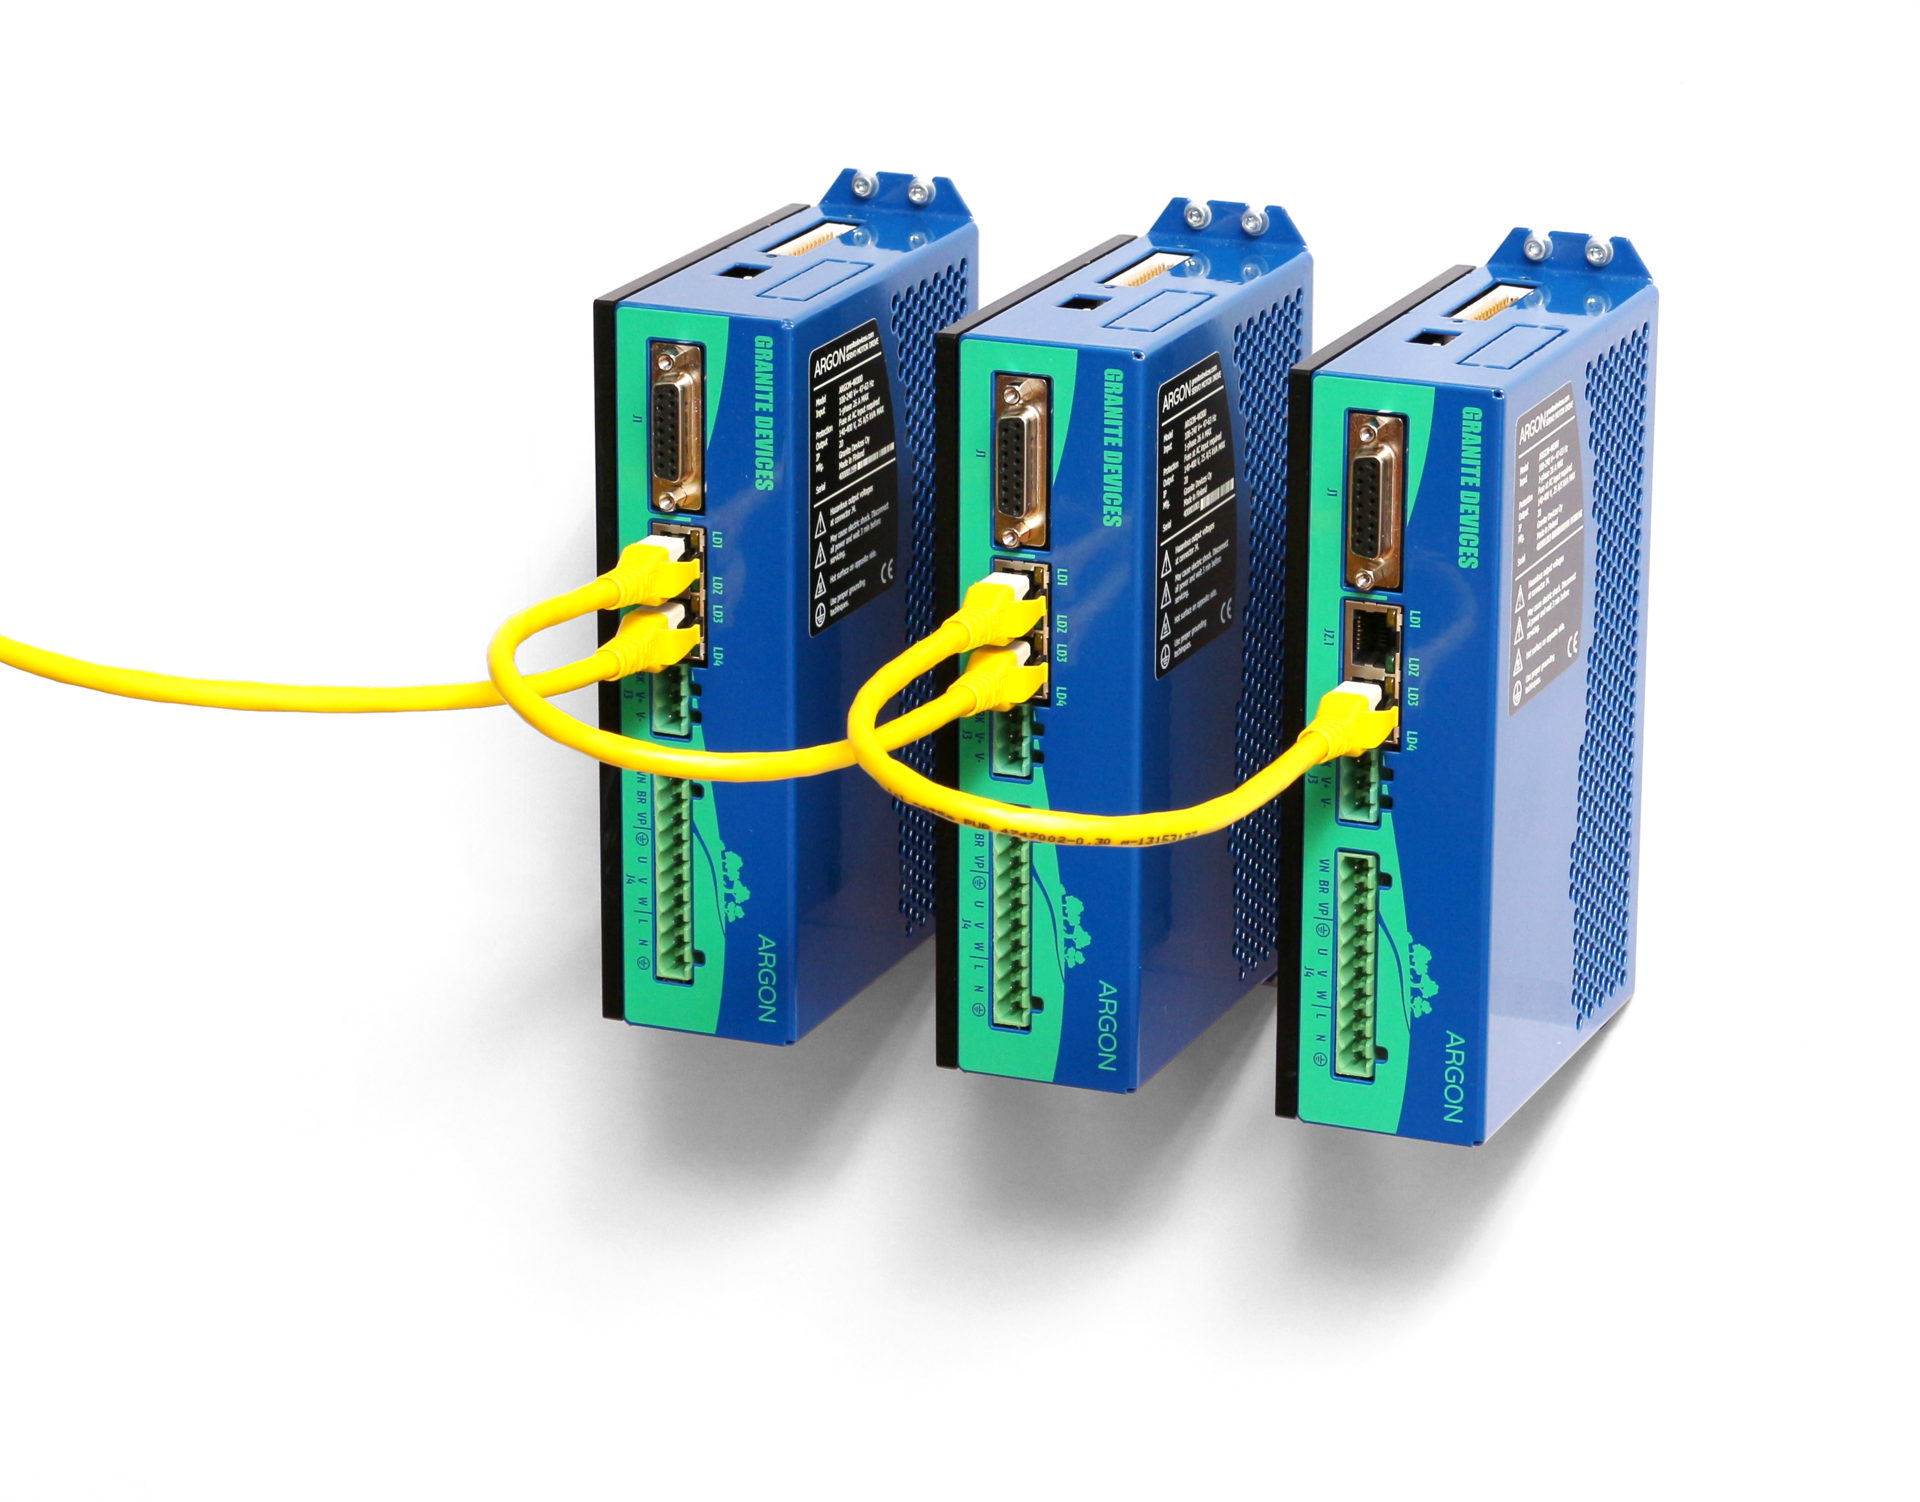
\includegraphics[height=2.5cm]{../figures/d2_servo_drives.png}\\
\credit{Tero Kontkanen, CC BY-SA 3.0, via Wikimedia Commons}
\end{columns}
\end{frame}

% ---------------------------------------------------------------------
\begin{frame}{Session 2.4 -- Summary}
\begin{keybox}[Key take-aways]
\begin{itemize}
  \item P sets speed, I removes steady-state error (adds lag), D adds phase lead (and noise) -- always filter D.
  \item Know the controller \hl{form} (parallel / ideal / series) and units before entering gains.
  \item Ziegler--Nichols is aggressive; model-based rules (SIMC, lambda) expose one robustness knob.
  \item Set-point weighting and feedforward improve tracking \emph{without} changing feedback robustness.
  \item Every saturating integrator needs \hl{anti-windup} (clamping or back-calculation).
  \item Servo drives: cascaded current / speed / position loops, tuned inside-out with bandwidth separation.
\end{itemize}
\end{keybox}
\end{frame}

% =====================================================================
\section{2.5 Stability and Performance Analysis}
% =====================================================================

\begin{frame}{Time-domain specifications}
\begin{columns}[T]
\column{.58\textwidth}
\centering
\begin{tikzpicture}
\begin{axis}[mkplot,width=8.4cm,height=5.6cm,xlabel={$\omega_nt$},ylabel={$y(t)$},xmin=0,xmax=14,ymin=0,ymax=1.4]
  \fill[mkPale] (axis cs:0,0.98) rectangle (axis cs:14,1.02);
  \addplot[mkBlue,very thick,domain=0:14,samples=250] {1-exp(-0.4*x)/sqrt(1-0.16)*sin(deg(sqrt(1-0.16)*x)+acos(0.4))};
  \addplot[mkGray,dashed,domain=0:14] {1};
  \draw[mkOrange,dashed] (axis cs:0.48,0)--(axis cs:0.48,0.1); \draw[mkOrange,dashed] (axis cs:1.94,0)--(axis cs:1.94,0.9);
  \draw[mkOrange,thick,<->] (axis cs:0.48,0.05)--(axis cs:1.94,0.05) node[midway,above,font=\tiny]{$t_r$};
  \draw[mkMid,dashed] (axis cs:3.43,0)--(axis cs:3.43,1.254);
  \node[font=\tiny,anchor=north west] at (axis cs:3.43,0.2) {$t_p=\pi/\omega_d$};
  \draw[mkOrange,thick,<->] (axis cs:4.2,1)--(axis cs:4.2,1.254) node[midway,right,font=\tiny]{$M_p=25.4\,\%$};
  \draw[mkMid,dashed] (axis cs:8.41,0)--(axis cs:8.41,0.98);
  \node[font=\tiny,anchor=north west] at (axis cs:8.41,0.45) {$t_s$ (2\,\%)};
  \node[font=\tiny,anchor=south east] at (axis cs:14,0.62) {$\zeta=0.4$};
\end{axis}
\end{tikzpicture}
\column{.40\textwidth}
\scriptsize
\begin{tabular}{@{}p{1.8cm}p{3.3cm}@{}}
\toprule
Measure & Definition\\
\midrule
Rise time $t_r$ & 10\,\% $\to$ 90\,\% of final value\\
Peak time $t_p$ & time of first maximum\\
Overshoot $M_p$ & $(y_{\max}-y_\infty)/y_\infty$\\
Settling time $t_s$ & last entry into $\pm2\,\%$ band\\
Steady-state error & $e_\infty=\lim_{t\to\infty}e(t)$\\
\bottomrule
\end{tabular}\\[4pt]
For $\zeta=0.4$: $\omega_nt_r=1.46$, $\omega_nt_p=3.43$, $\omega_nt_s=8.4$ (estimate $4/\zeta=10$).
\begin{notebox}
\scriptsize
\textbf{Transient} = response to the initial shock (poles). \textbf{Steady state} = what remains (system type, DC gain).
In servos also: following error during constant velocity, in-position window and settling time to it.
\end{notebox}
\end{columns}
\end{frame}

% ---------------------------------------------------------------------
\begin{frame}{Specifications versus damping ratio}
\begin{columns}[T]
\column{.5\textwidth}
\centering
\begin{tikzpicture}
\begin{axis}[mkplot,width=7.0cm,height=5.3cm,xlabel={damping ratio $\zeta$},ylabel={overshoot $M_p$ [\%]},
  xmin=0,xmax=1,ymin=0,ymax=100,axis y line*=left,legend style={at={(0.5,0.98)},anchor=north}]
  \addplot[mkOrange,very thick,domain=0.01:0.999,samples=120] {100*exp(-pi*x/sqrt(1-x^2))}; \label{pl:mp}
\end{axis}
\begin{axis}[mkplot,width=7.0cm,height=5.3cm,xmin=0,xmax=1,ymin=0,ymax=80,axis y line*=right,axis x line=none,
  ylabel={phase margin [deg]},grid=none,legend style={at={(0.97,0.5)},anchor=east}]
  \addlegendimage{/pgfplots/refstyle=pl:mp}\addlegendentry{$M_p$}
  \addplot[mkBlue,very thick,domain=0.01:1,samples=120] {atan(2*x/sqrt(sqrt(1+4*x^4)-2*x^2))}; \addlegendentry{PM (exact)}
  \addplot[mkSky,thick,dashed,domain=0:0.75] {100*x}; \addlegendentry{PM $\approx100\zeta$}
\end{axis}
\end{tikzpicture}
\column{.48\textwidth}
\scriptsize
For the closed-loop second-order system (exact formulas):
\begin{eqbox}
\[
M_p=e^{-\pi\zeta/\sqrt{1-\zeta^2}},\quad t_p=\frac{\pi}{\omega_n\sqrt{1-\zeta^2}},\quad t_s\approx\frac{4}{\zeta\omega_n}
\]
\end{eqbox}
Rules of thumb: $t_r\approx1.8/\omega_n$ (for $\zeta\approx0.5$), $\omega_b\approx\omega_n$ for $\zeta=0.707$.\\[3pt]
Link to the open loop $L(s)=\omega_n^2/(s(s+2\zeta\omega_n))$:
\[
\mathrm{PM}=\arctan\frac{2\zeta}{\sqrt{\sqrt{1+4\zeta^4}-2\zeta^2}}\approx100\,\zeta\ \text{[deg]}
\]
\begin{tabular}{@{}lccccc@{}}
\toprule
$\zeta$ & 0.3 & 0.4 & 0.5 & 0.6 & 0.7\\
\midrule
$M_p$ [\%] & 37 & 25 & 16 & 9.5 & 4.6\\
PM [deg] & 33 & 43 & 52 & 59 & 65\\
\bottomrule
\end{tabular}
\end{columns}
\end{frame}

% ---------------------------------------------------------------------
\begin{frame}{Steady-state error, system type and the final value theorem}
\begin{columns}[T]
\column{.48\textwidth}
\scriptsize
Unity feedback, $E(s)=S(s)R(s)=\dfrac{R(s)}{1+L(s)}$. If $sE(s)$ has all poles in the LHP:
\begin{eqbox}
\[
e_\infty=\lim_{t\to\infty}e(t)=\lim_{s\to0}s\,E(s)
\]
\end{eqbox}
\term{System type} $=$ number of integrators in $L(s)$: $L(s)=\dfrac{K\,\tilde L(s)}{s^N}$, $\tilde L(0)=1$.\\[3pt]
Error constants: $K_p=\lim_{s\to0}L$, $K_v=\lim_{s\to0}sL$, $K_a=\lim_{s\to0}s^2L$.\\[3pt]
\hl{Pitfall}: FVT applied to an unstable loop gives a finite but meaningless number.
\column{.5\textwidth}
\scriptsize
\begin{tabular}{@{}lccc@{}}
\toprule
Type $N$ & step $r=1$ & ramp $r=t$ & parabola $r=t^2/2$\\
\midrule
0 & $\dfrac{1}{1+K_p}$ & $\infty$ & $\infty$\\[4pt]
1 & 0 & $\dfrac{1}{K_v}$ & $\infty$\\[4pt]
2 & 0 & 0 & $\dfrac{1}{K_a}$\\
\bottomrule
\end{tabular}\\[4pt]
\textbf{Servo example}: position loop with P gain $K_{pp}=126$\,s$^{-1}$ around an ideal velocity loop $\Rightarrow$ $L=K_{pp}/s$, type 1.
At $v=0.2$\,m/s on a 10\,mm-pitch ball screw ($\dot\theta=126$\,rad/s):
following error $e_\infty=\dot\theta/K_v=126/126=1$\,rad $=1.6$\,mm.
\begin{itemize}
  \item Velocity feedforward removes it (makes the reference path ``type 2'').
  \item Integral action in the position loop adds a type but also phase lag.
\end{itemize}
\end{columns}
\end{frame}

% ---------------------------------------------------------------------
\begin{frame}{Routh--Hurwitz criterion}
\begin{columns}[T]
\column{.47\textwidth}
\scriptsize
Stability without computing roots: for $a_ns^n+a_{n-1}s^{n-1}+\dots+a_0$
\begin{itemize}
  \item Necessary: all coefficients present and of the same sign.
  \item Build the Routh array; number of \hl{sign changes} in the first column $=$ number of RHP roots.
\end{itemize}
Each new entry: $b_1=\dfrac{a_{n-1}a_{n-2}-a_na_{n-3}}{a_{n-1}}$, etc.\\[4pt]
\textbf{Example:} $L(s)=\dfrac{K}{s(s+2)(s+5)}$, unity feedback:
\[
1+L=0\;\Leftrightarrow\;s^3+7s^2+10s+K=0
\]
\column{.5\textwidth}
\centering
\small
\begin{tabular}{@{}c|cc@{}}
$s^3$ & 1 & 10\\
$s^2$ & 7 & $K$\\
$s^1$ & $\dfrac{70-K}{7}$ & 0\\[6pt]
$s^0$ & $K$ & \\
\end{tabular}\\[3mm]
\begin{keybox}[Result]
\scriptsize
Stable $\Leftrightarrow$ $0<K<70$.\\
At $K=70$: auxiliary polynomial $7s^2+70=0$ $\Rightarrow$ $s=\pm j\sqrt{10}=\pm j3.16$\,rad/s: the loop oscillates at the ultimate frequency.
For $K=20$: gain margin $70/20=3.5$ (10.9\,dB).
\end{keybox}
\scriptsize Limitation: yes/no answer, no direct information on damping or robustness; does not handle delays.
\end{columns}
\end{frame}

% ---------------------------------------------------------------------
\begin{frame}{Root locus: how closed-loop poles move with gain}
\begin{columns}[T]
\column{.52\textwidth}
\centering
\begin{tikzpicture}
\begin{axis}[mkplot,width=7.4cm,height=6.0cm,xlabel={Re},ylabel={Im},xmin=-9,xmax=3,ymin=-5,ymax=5,
  axis lines=middle,xlabel style={anchor=north east,at={(rel axis cs:1,0.5)}},
  ylabel style={anchor=south,at={(rel axis cs:0.75,1)}}]
  \addplot[mkGray,dashed,domain=-2.333:1.5] ({x},{(x+2.333)*1.732});
  \addplot[mkGray,dashed,domain=-2.333:1.5] ({x},{-(x+2.333)*1.732});
  \addplot[mkBlue,very thick] table[x=r1,y=i1] {data/rlocus.dat};
  \addplot[mkBlue,very thick] table[x=r2,y=i2] {data/rlocus.dat};
  \addplot[mkBlue,very thick] table[x=r3,y=i3] {data/rlocus.dat};
  \addplot[only marks,mark=x,mark size=3pt,mkNavy,very thick] coordinates {(0,0)(-2,0)(-5,0)};
  \addplot[only marks,mark=*,mark size=1.8pt,mkOrange] coordinates {(-0.561,1.757)(-0.561,-1.757)(-5.878,0)};
  \addplot[only marks,mark=square*,mark size=1.6pt,mkRed] coordinates {(0,3.162)(0,-3.162)};
  \node[font=\tiny,mkOrange,anchor=east] at (axis cs:-1.2,1.6) {$K=20$};
  \node[font=\tiny,mkRed,anchor=west] at (axis cs:0.15,3.162) {$K=70$};
  \node[font=\tiny,anchor=north east] at (axis cs:-0.95,-0.1) {$-0.88$};
\end{axis}
\end{tikzpicture}
\column{.46\textwidth}
\scriptsize
Locus of the roots of $1+K\,\tilde L(s)=0$ for $K:0\to\infty$; here $\tilde L=\dfrac{1}{s(s+2)(s+5)}$.
\begin{itemize}
  \item Starts at open-loop \term{poles} ($K=0$), ends at open-loop zeros or at infinity.
  \item On the real axis left of an odd number of poles+zeros.
  \item Asymptotes: centroid $\sigma_a=\frac{0-2-5}{3}=-2.33$, angles $\pm60^\circ,180^\circ$.
  \item Break-away: $\frac{d}{ds}[s(s+2)(s+5)]=0$ $\Rightarrow$ $s=-0.88$ ($K=4.06$).
  \item $j\omega$-crossing at $\pm j3.16$, $K=70$ -- consistent with Routh.
  \item $K=20$: poles $-0.56\pm j1.76$ ($\zeta=0.30$) and $-5.88$.
\end{itemize}
\hl{Use}: see at a glance how gain trades speed for damping, and why more gain eventually destabilises a $\ge3$rd-order loop.
\end{columns}
\end{frame}

% ---------------------------------------------------------------------
\begin{frame}{Nyquist criterion}
\begin{columns}[T]
\column{.5\textwidth}
\centering
\begin{tikzpicture}
\begin{axis}[mkplot,width=7.2cm,height=6.0cm,xlabel={Re $L(j\omega)$},ylabel={Im $L(j\omega)$},
  xmin=-2.5,xmax=1,ymin=-2.5,ymax=1,axis equal image,axis lines=middle,
  xlabel style={anchor=north east,at={(rel axis cs:1,0.71)}},ylabel style={anchor=south,at={(rel axis cs:0.71,1)}}]
  \draw[mkOrange,thick,dashed] (axis cs:-1,0) circle [radius=0.472];
  \addplot[mkBlue,very thick] table[x=re,y=im] {data/nyquist.dat};
  \addplot[mkSky,thick,dashed] table[x=re,y=imneg] {data/nyquist.dat};
  \addplot[only marks,mark=+,mark size=4pt,mkRed,very thick] coordinates {(-1,0)};
  \addplot[only marks,mark=*,mark size=1.5pt,mkNavy] coordinates {(-0.2857,0)};
  \draw[mkSky] (axis cs:0,0) circle [radius=1];
  \node[font=\tiny,mkRed,anchor=north] at (axis cs:-1,-0.05) {$-1$};
  \node[font=\tiny,anchor=south] at (axis cs:-0.25,0.03) {$-1/\mathrm{GM}$};
  \node[font=\tiny,mkOrange,anchor=north] at (axis cs:-1,-0.48) {$1/M_s$};
  \node[font=\tiny,mkBlue,anchor=west] at (axis cs:-1.5,-2.2) {$\omega\uparrow$};
\end{axis}
\end{tikzpicture}
\column{.48\textwidth}
\scriptsize
Plot $L(j\omega)$ for $\omega:-\infty\to\infty$ (indent around poles on the $j\omega$-axis).
\begin{eqbox}
\[
Z=N+P
\]
\end{eqbox}
$Z$: closed-loop RHP poles, $P$: open-loop RHP poles, $N$: clockwise encirclements of $-1$.
\begin{itemize}
  \item Stable open loop ($P=0$): closed loop stable $\Leftrightarrow$ no encirclement of $-1$.
  \item Here $L=20/(s(s+2)(s+5))$: crosses the real axis at $-20/70=-0.286$ $\Rightarrow$ GM $=3.5$.
  \item Unit circle crossing gives the phase margin.
  \item \hl{Distance to $-1$} is the true robustness measure: $\min_\omega|1+L|=1/M_s$.
  \item Works with dead time $e^{-sT_d}$ and with measured FRF data -- no model needed.
\end{itemize}
\end{columns}
\end{frame}

% ---------------------------------------------------------------------
\begin{frame}{Gain and phase margins on the Bode diagram}
\begin{columns}[T]
\column{.56\textwidth}
\centering
\begin{tikzpicture}
\begin{groupplot}[group style={group size=1 by 2,vertical sep=4mm,x descriptions at=edge bottom},
  mkplot,width=8.0cm,height=3.9cm,xmode=log,xmin=0.1,xmax=100]
\nextgroupplot[ylabel={$|L|$ [dB]},ymin=-60,ymax=50]
  \addplot[mkBlue,very thick] table[x=w,y=mag] {data/loop_bode.dat};
  \addplot[mkGray,dashed,domain=0.1:100] {0};
  \draw[mkOrange,very thick,<->] (axis cs:3.17,0)--(axis cs:3.17,-10.9) node[midway,right,font=\tiny]{GM $=10.9$\,dB};
  \fill[mkNavy] (axis cs:1.515,0) circle (1.5pt);
  \node[font=\tiny,anchor=south west] at (axis cs:1.55,0.5) {$\omega_c=1.52$};
\nextgroupplot[ylabel={$\angle L$ [deg]},xlabel={$\omega$ [rad/s]},ymin=-270,ymax=-80,ytick={-270,-225,-180,-135,-90}]
  \addplot[mkBlue,very thick] table[x=w,y=ph] {data/loop_bode.dat};
  \addplot[mkGray,dashed,domain=0.1:100] {-180};
  \draw[mkOrange,very thick,<->] (axis cs:1.515,-180)--(axis cs:1.515,-144) node[midway,left,font=\tiny]{PM $=36^\circ$};
  \fill[mkNavy] (axis cs:3.17,-180) circle (1.5pt);
  \node[font=\tiny,anchor=north west] at (axis cs:3.2,-182) {$\omega_{180}=3.16$};
\end{groupplot}
\end{tikzpicture}
\column{.42\textwidth}
\scriptsize
\begin{defbox}[Definitions]
\scriptsize
Crossover $\omega_c$: $|L(j\omega_c)|=1$; \quad PM $=180^\circ+\angle L(j\omega_c)$\\
Phase crossover $\omega_{180}$: $\angle L=-180^\circ$; \quad GM $=1/|L(j\omega_{180})|$
\end{defbox}
\begin{itemize}
  \item GM: how much the gain may increase (motor $k_t$, inertia drop) before instability.
  \item PM: how much extra \hl{phase lag} is tolerable. A pure delay $T_d$ costs $\omega_cT_d$ rad: delay margin $=\mathrm{PM}/\omega_c$.
  \item Example $K=20$: PM $=36^\circ$ $\Rightarrow$ delay margin $=0.628/1.515=0.41$\,s.
  \item Typical targets: PM $45$--$60^\circ$, GM $\ge6$--$10$\,dB.
  \item Margins can mislead for loops with several crossings -- check $M_s$.
\end{itemize}
\end{columns}
\end{frame}

% ---------------------------------------------------------------------
\begin{frame}{Sensitivity functions, $M_s$ and bandwidth}
\begin{columns}[T]
\column{.5\textwidth}
\centering
\begin{tikzpicture}
\begin{axis}[mkplot,width=7.0cm,height=4.4cm,xmode=log,xmin=0.01,xmax=100,ymin=-40,ymax=15,
  xlabel={$\omega$ [rad/s]},ylabel={magnitude [dB]},legend pos=south west]
  \addplot[mkOrange,very thick] table[x=w,y=S] {data/loop_bode.dat}; \addlegendentry{$|S|$}
  \addplot[mkBlue,very thick] table[x=w,y=T] {data/loop_bode.dat}; \addlegendentry{$|T|$}
  \addplot[mkGray,dashed,domain=0.01:100] {-3};
  \node[font=\tiny,mkOrange,anchor=south west] at (axis cs:2.2,6.6) {$M_s=2.12$ (6.5\,dB)};
  \node[font=\tiny,mkBlue,anchor=south west] at (axis cs:2.6,-3) {$\omega_b=2.6$};
\end{axis}
\end{tikzpicture}
\begin{tikzpicture}
\begin{axis}[mkplot,width=7.0cm,height=3.6cm,xmin=0,xmax=12,ymin=0,ymax=1.9,xlabel={time [s]},ylabel={$y$},
  legend pos=north east,legend columns=3]
  \addplot[mkSky,thick] table[x=t,y=k10] {data/loop_step.dat}; \addlegendentry{$K=10$}
  \addplot[mkBlue,very thick] table[x=t,y=k20] {data/loop_step.dat}; \addlegendentry{$20$}
  \addplot[mkRed,thick] table[x=t,y=k50] {data/loop_step.dat}; \addlegendentry{$50$}
\end{axis}
\end{tikzpicture}
\column{.48\textwidth}
\scriptsize
\begin{itemize}
  \item $S=\frac{1}{1+L}$: disturbance/error response; $T=\frac{L}{1+L}$: tracking and noise response; $S+T=1$.
  \item \term{Bandwidth} $\omega_b$: where $|T|$ falls to $-3$\,dB; typically $\omega_c<\omega_b<2\omega_c$.
  \item $M_s=\max_\omega|S(j\omega)|$; $|S|>1$ means feedback \hl{amplifies} disturbances there.
\end{itemize}
\begin{eqbox}
\[
\mathrm{GM}\ge\frac{M_s}{M_s-1},\qquad \mathrm{PM}\ge2\arcsin\frac{1}{2M_s}
\]
\end{eqbox}
\begin{itemize}
  \item $M_s=2$: GM $\ge6$\,dB, PM $\ge29^\circ$. $M_s=1.4$: GM $\ge10.9$\,dB, PM $\ge41^\circ$.
  \item Recommended $M_s=1.2$--$2.0$ [\AA str\"om \& H\"agglund, 2006].
  \item \hl{Waterbed effect} (Bode integral): $\int_0^\infty\ln|S(j\omega)|\,d\omega=0$ for stable $L$ with relative degree $\ge2$ -- pushing $|S|$ down somewhere raises it elsewhere.
\end{itemize}
\end{columns}
\end{frame}

% ---------------------------------------------------------------------
\begin{frame}{Session 2.5 -- Summary and design targets}
\begin{columns}[T]
\column{.5\textwidth}
\begin{keybox}[Key take-aways]
\scriptsize
\begin{itemize}
  \item Specs: $t_r$, $t_p$, $M_p$, $t_s$, $e_\infty$; for 2nd order all follow from $\zeta$ and $\omega_n$.
  \item System type decides steady-state error; FVT only for stable loops.
  \item Routh: yes/no stability and gain limits; root locus: pole movement with gain.
  \item Nyquist: encirclements of $-1$; works with delays and measured FRFs.
  \item Margins PM, GM and above all $M_s$ quantify robustness; $\omega_c$, $\omega_b$ quantify speed.
\end{itemize}
\end{keybox}
\column{.47\textwidth}
\scriptsize
\textbf{Typical design targets (servo / process)}\\[2pt]
\begin{tabular}{@{}lc@{}}
\toprule
Quantity & Target\\
\midrule
Phase margin PM & 45--60$^\circ$\\
Gain margin GM & 6--12\,dB\\
Max.\ sensitivity $M_s$ & 1.3--2.0\\
Max.\ compl.\ sens.\ $M_t$ & $\le1.3$\ldots1.5\\
Overshoot (position step) & 0--5\,\% (often 0)\\
$\omega_c$ vs.\ first resonance & $\omega_c<\omega_r/3$ (w/o notch)\\
$\omega_c$ vs.\ sample rate & $\omega_c<\omega_s/20$ roughly\\
\bottomrule
\end{tabular}\\[3pt]
Our example $K=20$: PM $36^\circ$, $M_s=2.12$ $\Rightarrow$ too aggressive; $K\approx10$ would meet the targets.
\end{columns}
\end{frame}

% =====================================================================
\section{Wrap-up}
% =====================================================================
\begin{frame}{Day summary}
\begin{columns}[T]
\column{.5\textwidth}
\begin{defbox}[Modelling chain]
\scriptsize
nonlinear physics $\xrightarrow{\text{Jacobian}}$ $(A,B,C,D)$ $\xrightarrow{C(sI-A)^{-1}B+D}$ $G(s)$ $\xrightarrow{s=j\omega}$ Bode / Nyquist\\[3pt]
\ldots{} and in the lab: step test / FRF $\to$ FOPDT, 2nd order, non-parametric $\hat G(j\omega)$ + uncertainty $\Delta(j\omega)$.
\end{defbox}
\begin{defbox}[Control chain]
\scriptsize
PID (form, filter, set-point weights) + anti-windup + feedforward, cascaded current $\to$ speed $\to$ position.
\end{defbox}
\column{.47\textwidth}
\begin{keybox}[Ten numbers to remember]
\scriptsize
\begin{tabular}{@{}ll@{}}
63\,\% & first-order step at $t=\tau$\\
$\zeta=0.7$ & $\approx$\,5\,\% overshoot, PM $\approx65^\circ$\\
$-20$\,dB/dec & per pole; $-40$\,dB/dec per pair\\
$1/(2\zeta)$ & resonance peak at $\omega_n$\\
$\gamma^2>0.8$ & trustworthy FRF\\
$N=5$--$20$ & derivative filter\\
4--10$\times$ & cascade bandwidth separation\\
45--60$^\circ$ & phase margin\\
6--12\,dB & gain margin\\
$M_s\le2$ & robustness\\
\end{tabular}
\end{keybox}
\end{columns}
\end{frame}

% ---------------------------------------------------------------------
\begin{frame}{Preview of Day 3}
\begin{columns}[T]
\column{.55\textwidth}
\textbf{\small Day 3 -- Control: filters, modern, adaptive and discrete control + servo architecture}\\[2mm]
\scriptsize
\begin{itemize}
  \item Filters in the loop: low-pass, high-pass and notch filters, their phase lag and placement; lead/lag compensators.
  \item Modern control: state feedback, pole placement, controllability, observability, observers.
  \item Adaptive and robust control: parameter variation, MRAC structure, Lyapunov reasoning, goals of robust control.
  \item Discrete-time control: sampling, zero-order hold, discretisation, computation delay, stability in the $z$-plane.
  \item Start of servo systems: architecture, power electronics -- inverter and DC link.
\end{itemize}
\column{.42\textwidth}
\begin{notebox}
\scriptsize
\textbf{Bridge from today}\\
\checkitem\ State space $(A,B,C,D)$ $\to$ state feedback and observers.\\
\checkitem\ Phase margin and $M_s$ $\to$ the phase cost of every filter.\\
\checkitem\ Delay margin $\to$ sampling and computation delay.\\
\checkitem\ Uncertainty $\Delta(j\omega)$ $\to$ robust and adaptive control.
\end{notebox}
\centering
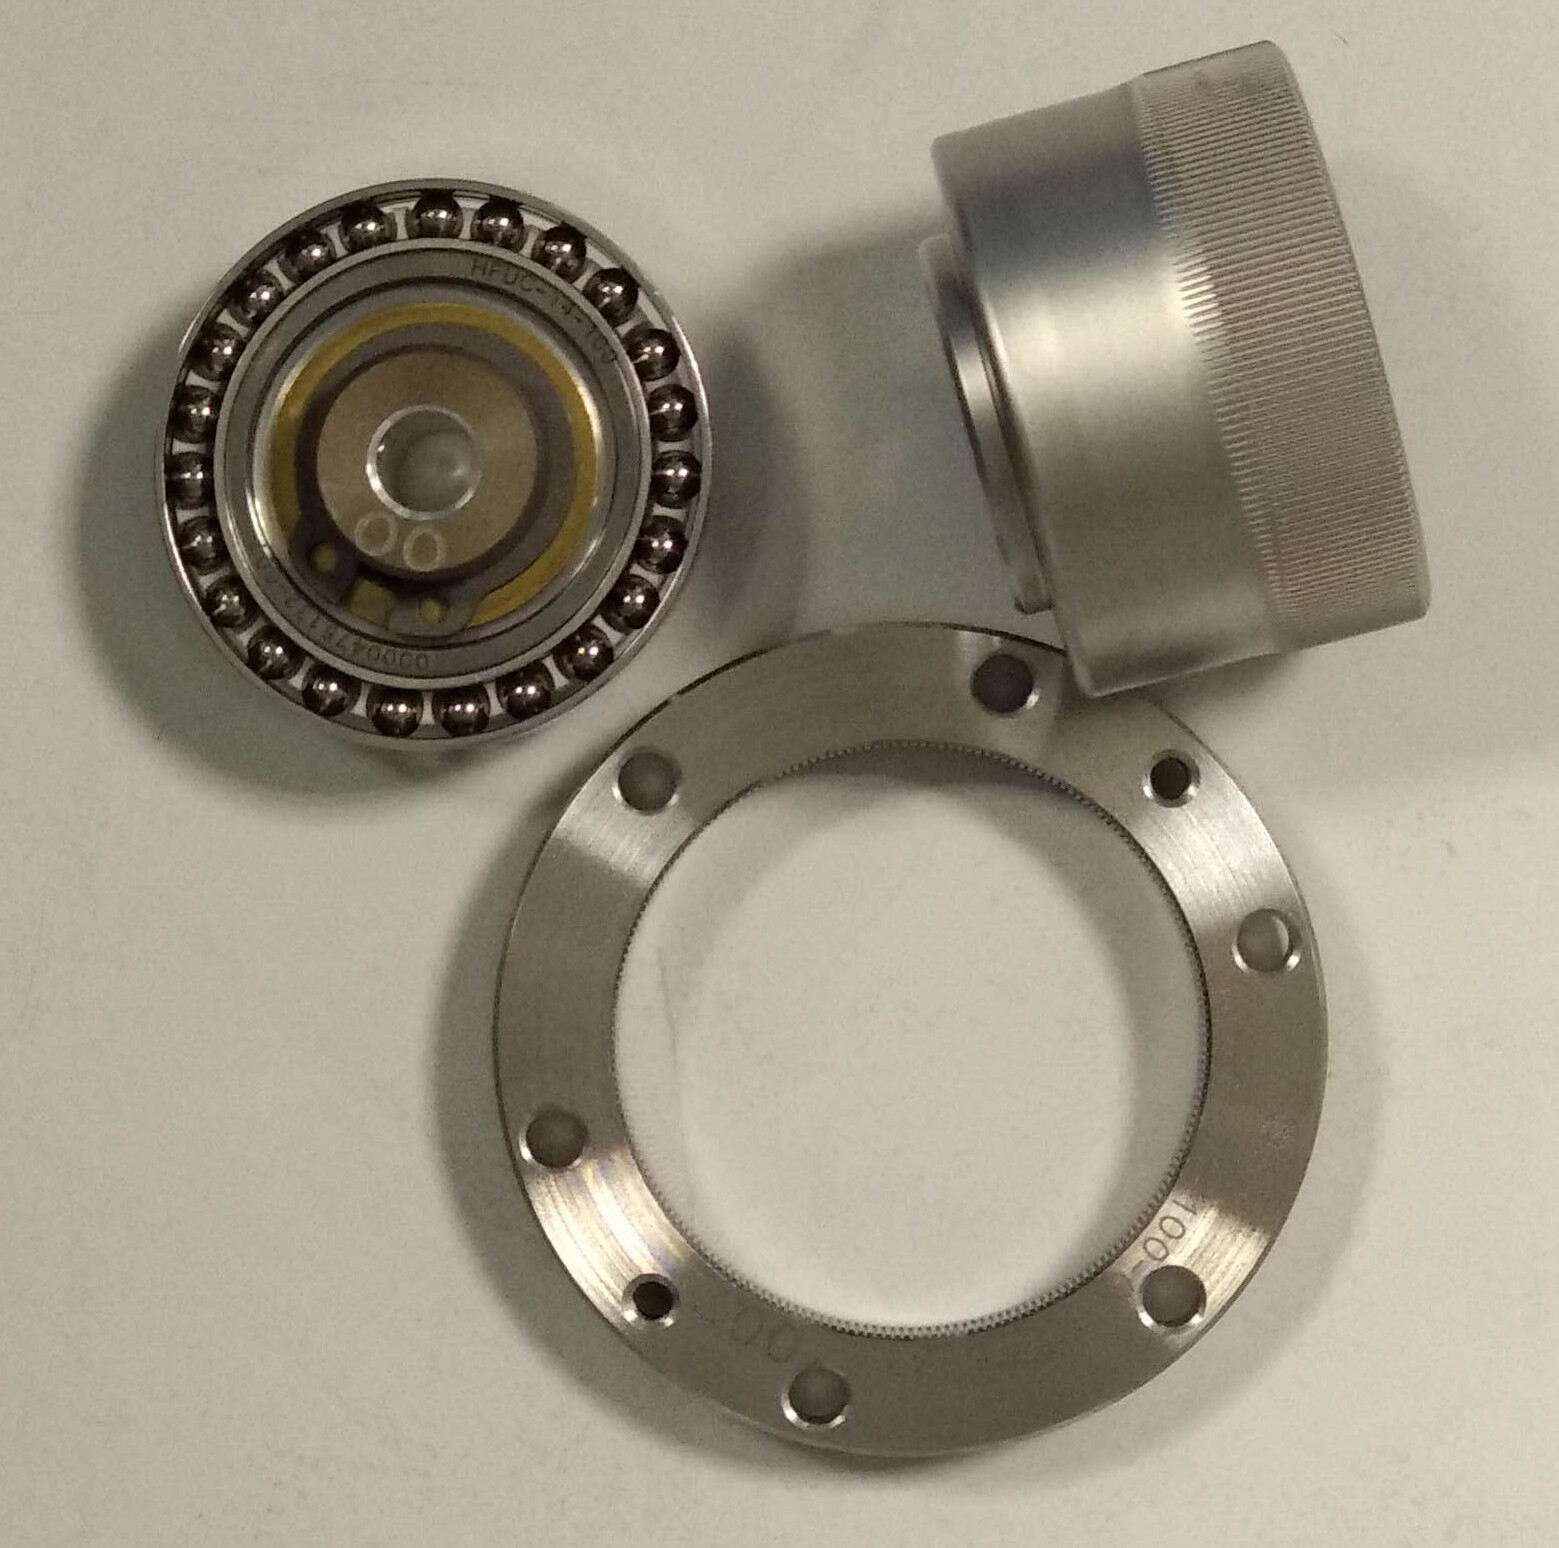
\includegraphics[height=2.6cm]{../figures/d2_harmonic_drive.jpg}\\
\credit{Pieceofmetalwork, CC BY-SA 4.0, via Wikimedia Commons}\\
\scriptsize Strain-wave gear: compliant transmissions motivate notch filters and observers.
\end{columns}
\end{frame}

% ---------------------------------------------------------------------
\begin{frame}{Figure credits}
\fontsize{7}{8.5}\selectfont
All other drawings and plots: own work (TikZ / pgfplots; numerical data from \texttt{day2/data/gen\_data.py}).\\[2mm]
\begin{tabularx}{\textwidth}{@{}lXll@{}}
\toprule
File & Source (Wikimedia Commons) & Author & License\\
\midrule
d2\_backlash.png & File:Backlash.svg & GearHeads, Slashme & CC BY-SA 3.0\\
d2\_solenoid.jpg & File:Solenoid-with-core.JPG & Svjo & CC BY-SA 3.0\\
d2\_bode\_portrait.png & File:Hendrik Wade Bode.png & unknown author & Public domain\\
d2\_signal\_analyzer.jpg & File:3562A Dynamic Signal Analyzer HP.jpg & Loxyger & CC BY 4.0\\
d2\_governor.jpg & File:Centrifugal governor (Heat Engines, 1913).jpg & Andy Dingley (scan) & Public domain\\
d2\_pid\_controllers.jpg & File:Industrial PID controllers - front display.jpg & Bitjungle & CC BY-SA 4.0\\
d2\_servo\_drives.png & File:Servo motor drive.png & Tero Kontkanen & CC BY-SA 3.0\\
d2\_harmonic\_drive.jpg & File:Harmonic Drive AG strain wave gear set.jpg & Pieceofmetalwork & CC BY-SA 4.0\\
\bottomrule
\end{tabularx}
\end{frame}

% ---------------------------------------------------------------------
\begin{frame}{References}
\fontsize{7}{8.5}\selectfont
\begin{columns}[T]
\column{.5\textwidth}
\begin{itemize}
  \item K.\ Ogata, \emph{Modern Control Engineering}, 5th ed., Prentice Hall, 2010.
  \item G.\,F.\ Franklin, J.\,D.\ Powell, A.\ Emami-Naeini, \emph{Feedback Control of Dynamic Systems}, 8th ed., Pearson, 2019.
  \item K.\,J.\ \AA str\"om, R.\,M.\ Murray, \emph{Feedback Systems: An Introduction for Scientists and Engineers}, Princeton Univ.\ Press, 2008.
  \item K.\,J.\ \AA str\"om, T.\ H\"agglund, \emph{Advanced PID Control}, ISA, 2006.
  \item G.\ Ellis, \emph{Control System Design Guide}, 4th ed., Butterworth-Heinemann, 2012.
  \item J.-J.\,E.\ Slotine, W.\ Li, \emph{Applied Nonlinear Control}, Prentice Hall, 1991.
  \item L.\ Ljung, \emph{System Identification: Theory for the User}, 2nd ed., Prentice Hall, 1999.
\end{itemize}
\column{.5\textwidth}
\begin{itemize}
  \item R.\ Pintelon, J.\ Schoukens, \emph{System Identification: A Frequency Domain Approach}, 2nd ed., Wiley/IEEE Press, 2012.
  \item S.\ Skogestad, ``Simple analytic rules for model reduction and PID controller tuning,'' \emph{J.\ Process Control} 13, 291--309, 2003.
  \item J.\,G.\ Ziegler, N.\,B.\ Nichols, ``Optimum settings for automatic controllers,'' \emph{Trans.\ ASME} 64, 759--768, 1942.
  \item B.\ Armstrong-H\'elouvry, P.\ Dupont, C.\ Canudas de Wit, ``A survey of models, analysis tools and compensation methods for the control of machines with friction,'' \emph{Automatica} 30(7), 1994.
  \item K.\ Zhou, J.\,C.\ Doyle, \emph{Essentials of Robust Control}, Prentice Hall, 1998.
  \item W.\ Leonhard, \emph{Control of Electrical Drives}, 3rd ed., Springer, 2001.
  \item J.\,C.\ Maxwell, ``On governors,'' \emph{Proc.\ Royal Society of London} 16, 270--283, 1868.
\end{itemize}
\end{columns}
\end{frame}

\end{document}
